\documentclass[preprint]{elsarticle}
%DIF LATEXDIFF DIFFERENCE FILE
%DIF DEL ../main.tex     Tue Sep 21 08:30:00 2021
%DIF ADD revisions.tex   Thu Sep 23 08:18:09 2021

\usepackage{multirow}
\usepackage{lineno}
\usepackage{xspace}
\usepackage{threeparttable}
\usepackage{caption}
\usepackage{subcaption}
\modulolinenumbers[5]

%% Journal name here
\journal{EPJ N}

%% `Elsevier LaTeX' style
\bibliographystyle{elsarticle-num}
%%%%%%%%%%%%%%%%%%%%%%%

%%%% packages and definitions (optional)
\usepackage{placeins}
\usepackage{booktabs} % nice rules (thick lines) for tables
\usepackage{microtype} % improves typography for PDF
\usepackage{hhline}
\usepackage{amsmath}

\usepackage{threeparttable, tablefootnote}

\usepackage{tabularx}

%DIF 29a29
 %DIF > 
%DIF -------
%% Special typesetting for Cyclus
\newcommand{\Cyclus}{\textsc{Cyclus}\xspace}%
\newcommand{\Cycamore}{\textsc{Cycamore}\xspace}%
\graphicspath{{images/}}

% tikz %
\usepackage{tikz}
\usetikzlibrary{shapes.geometric, arrows}
\usetikzlibrary{positioning, arrows, decorations, shapes}

\tikzstyle{facility} = [rectangle, rounded corners, minimum width=2cm, minimum height=0.75cm,text centered, draw=black, fill=blue!30]
\tikzstyle{transition} = [rectangle, rounded corners, minimum width=2cm, minimum height=0.75cm,text centered, draw=black, fill=red!30]
\tikzstyle{arrow} = [thick,->,>=stealth]

% hyperref %
\usepackage[hidelinks]{hyperref}
% after hyperref %
\usepackage{cleveref}
\usepackage{datatool}
\usepackage[acronym,toc]{glossaries}
\newacronym[longplural={metric tons of heavy metal}]{MTHM}{MTHM}{metric ton of heavy metal}
\newacronym{ABM}{ABM}{agent-based modeling}
\newacronym{ACDIS}{ACDIS}{Program in Arms Control \& Domestic and International Security}
\newacronym{AHTR}{AHTR}{Advanced High Temperature Reactor}
\newacronym{ANDRA}{ANDRA}{Agence Nationale pour la gestion des D\'echets RAdioactifs, the French National Agency for Radioactive Waste Management}
\newacronym{APP}{APP}{Abbott Power Plant}
\newacronym{ANL}{ANL}{Argonne National Laboratory}
\newacronym{API}{API}{application programming interface}
\newacronym{ARCH}{ARCH}{autoregressive conditional heteroskedastic}
\newacronym{ARE}{ARE}{Aircraft Reactor Experiment}
\newacronym{ARFC}{ARFC}{Advanced Reactors and Fuel Cycles}
\newacronym{ARMA}{ARMA}{autoregressive moving average}
\newacronym{ASME}{ASME}{American Society of Mechanical Engineers}
\newacronym{ATWS}{ATWS}{Anticipated Transient Without Scram}
\newacronym{BDBE}{BDBE}{Beyond Design Basis Event}
\newacronym{BIDS}{BIDS}{Berkeley Institute for Data Science}
\newacronym{BOL}{BOL}{Beginning-of-Life}
\newacronym{BSD}{BSD}{Berkeley Software Distribution}
\newacronym{CAFCA}{CAFCA}{ Code for Advanced Fuel Cycles Assessment }
\newacronym{CASL}{CASL}{Consortium for Advanced Simulation of Light Water Reactors}
\newacronym{CDTN}{CDTN}{Centro de Desenvolvimento da Tecnologia Nuclear}
\newacronym{CEA}{CEA}{Commissariat \`a l'\'Energie Atomique et aux \'Energies Alternatives}
\newacronym{CI}{CI}{continuous integration}
\newacronym{CNEC}{CNEC}{Consortium for Nonproliferation Enabling Capabilities}
\newacronym{CNEN}{CNEN}{Comiss\~{a}o Nacional de Energia Nuclear}
\newacronym{CNERG}{CNERG}{Computational Nuclear Engineering Research Group}
\newacronym{COSI}{COSI}{Commelini-Sicard}
\newacronym{COTS}{COTS}{commercial, off-the-shelf}
\newacronym{CSNF}{CSNF}{commercial spent nuclear fuel}
\newacronym{CTAH}{CTAHs}{Coiled Tube Air Heaters}
\newacronym{CUBIT}{CUBIT}{CUBIT Geometry and Mesh Generation Toolkit}
\newacronym{CURIE}{CURIE}{Centralized Used Fuel Resource for Information Exchange}
\newacronym{DAG}{DAG}{directed acyclic graph}
\newacronym{DANESS}{DANESS}{Dynamic Analysis of Nuclear Energy System Strategies}
\newacronym{DBE}{DBE}{Design Basis Event}
\newacronym{DESAE}{DESAE}{Dynamic Analysis of Nuclear Energy Systems Strategies}
\newacronym{DHS}{DHS}{Department of Homeland Security}
\newacronym{DOE}{DOE}{Department of Energy}
\newacronym{DOE-NE}{DOE-NE}{U.S. Department of Energy Office of Nuclear Energy}
\newacronym{DRACS}{DRACS}{Direct Reactor Auxiliary Cooling System}
\newacronym{DRE}{DRE}{dynamic resource exchange}
\newacronym{DSNF}{DSNF}{DOE spent nuclear fuel}
\newacronym{DYMOND}{DYMOND}{Dynamic Model of Nuclear Development }
\newacronym{EBS}{EBS}{Engineered Barrier System}
\newacronym{EDZ}{EDZ}{Excavation Disturbed Zone}
\newacronym{EFPD}{EFPD}{effective full power days}
\newacronym{EIA}{EIA}{U.S. Energy Information Administration}
\newacronym{EOL}{EOL}{end of life}
\newacronym{EPA}{EPA}{Environmental Protection Agency}
\newacronym{EP}{EP}{Engineering Physics}
\newacronym{ES}{E\&S}{Evaluation and Screening}
\newacronym{EG}{EG}{evaluation group}
\newacronym{FCO}{FCO}{Fuel Cycle Options}
\newacronym{FCT}{FCT}{Fuel Cycle Technology}
\newacronym{FCWMD}{FCWMD}{Fuel Cycle and Waste Management Division}
\newacronym{FEHM}{FEHM}{Finite Element Heat and Mass Transfer}
\newacronym{FEPs}{FEPs}{Features, Events, and Processes}
\newacronym{FHR}{FHR}{Fluoride-Salt-Cooled High-Temperature Reactor}
\newacronym{FLiBe}{FLiBe}{Fluoride-Lithium-Beryllium}
\newacronym{GCAM}{GCAM}{Global Change Assessment Model}
\newacronym{GDSE}{GDSE}{Generic Disposal System Environment}
\newacronym{GDSM}{GDSM}{Generic Disposal System Model}
\newacronym{GENIUSv1}{GENIUSv1}{Global Evaluation of Nuclear Infrastructure Utilization Scenarios, Version 1}
\newacronym{GENIUSv2}{GENIUSv2}{Global Evaluation of Nuclear Infrastructure Utilization Scenarios, Version 2}
\newacronym{GENIUS}{GENIUS}{Global Evaluation of Nuclear Infrastructure Utilization Scenarios}
\newacronym{GPAM}{GPAM}{Generic Performance Assessment Model}
\newacronym{GRSAC}{GRSAC}{Graphite Reactor Severe Accident Code}
\newacronym{GUI}{GUI}{graphical user interface}
\newacronym{HALEU}{HALEU}{High-Assay Low-Enriched Uranium}
\newacronym{HEU}{HEU}{High-Enriched Uranium}
\newacronym{HLW}{HLW}{high level waste}
\newacronym{HPC}{HPC}{high-performance computing}
\newacronym{HTC}{HTC}{high-throughput computing}
\newacronym{HTGR}{HTGR}{High Temperature Gas-Cooled Reactor}
\newacronym{IAEA}{IAEA}{International Atomic Energy Agency}
\newacronym{IEMA}{IEMA}{Illinois Emergency Mangament Agency}
\newacronym{INL}{INL}{Idaho National Laboratory}
\newacronym{IPRR1}{IRP-R1}{Instituto de Pesquisas Radioativas Reator 1}
\newacronym{IRP}{IRP}{Integrated Research Project}
\newacronym{ISFSI}{ISFSI}{Independent Spent Fuel Storage Installation}
\newacronym{ISRG}{ISRG}{Independent Student Research Group}
\newacronym{JFNK}{JFNK}{Jacobian-Free Newton Krylov}
\newacronym{LANL}{LANL}{Los Alamos National Laboratory}
\newacronym{LBNL}{LBNL}{Lawrence Berkeley National Laboratory}
\newacronym{LCOE}{LCOE}{levelized cost of electricity}
\newacronym{LDRD}{LDRD}{laboratory directed research and development}
\newacronym{LEU}{LEU}{Low-Enriched Uranium}
\newacronym{LFR}{LFR}{Lead-Cooled Fast Reactor}
\newacronym{LGPL}{LGPL}{Lesser GNU Public License}
\newacronym{LLNL}{LLNL}{Lawrence Livermore National Laboratory}
\newacronym{LMFBR}{LMFBR}{Liquid-Metal-cooled Fast Breeder Reactor}
\newacronym{LOFC}{LOFC}{Loss of Forced Cooling}
\newacronym{LOHS}{LOHS}{Loss of Heat Sink}
\newacronym{LOLA}{LOLA}{Loss of Large Area}
\newacronym{LP}{LP}{linear program}
\newacronym{LWR}{LWR}{Light Water Reactor}
\newacronym{MARKAL}{MARKAL}{MARKet and ALlocation}
\newacronym{MA}{MA}{minor actinide}
\newacronym{MCNP}{MCNP}{Monte Carlo N-Particle code}
\newacronym{MILP}{MILP}{mixed-integer linear program}
\newacronym{MIT}{MIT}{the Massachusetts Institute of Technology}
\newacronym{MMR}{MMR\textsuperscript{TM}}{Micro Modular Reactor\textsuperscript{TM}}
\newacronym{MOAB}{MOAB}{Mesh-Oriented datABase}
\newacronym{MOOSE}{MOOSE}{Multiphysics Object-Oriented Simulation Environment}
\newacronym{MOX}{MOX}{mixed oxide}
\newacronym{MSBR}{MSBR}{Molten Salt Breeder Reactor}
\newacronym{MSRE}{MSRE}{Molten Salt Reactor Experiment}
\newacronym{MSR}{MSR}{Molten Salt Reactor}
\newacronym{NAGRA}{NAGRA}{National Cooperative for the Disposal of Radioactive Waste}
\newacronym{NCSA}{NCSA}{National Center for Supercomputing Applications}
\newacronym{NEAMS}{NEAMS}{Nuclear Engineering Advanced Modeling and Simulation}
\newacronym{NEUP}{NEUP}{Nuclear Energy University Programs}
\newacronym{NFCSim}{NFCSim}{Nuclear Fuel Cycle Simulator}
\newacronym{NFC}{NFC}{Nuclear Fuel Cycle}
\newacronym{NGNP}{NGNP}{Next Generation Nuclear Plant}
\newacronym{NMWPC}{NMWPC}{Nuclear MW Per Capita}
\newacronym{NNSA}{NNSA}{National Nuclear Security Administration}
\newacronym{NPRE}{NPRE}{Department of Nuclear, Plasma, and Radiological Engineering}
\newacronym{NQA1}{NQA-1}{Nuclear Quality Assurance - 1}
\newacronym{NRC}{NRC}{Nuclear Regulatory Commission}
\newacronym{NSF}{NSF}{National Science Foundation}
\newacronym{NSSC}{NSSC}{Nuclear Science and Security Consortium}
\newacronym{NU}{NU}{natural uranium}
\newacronym{NUWASTE}{NUWASTE}{Nuclear Waste Assessment System for Technical Evaluation}
\newacronym{NWF}{NWF}{Nuclear Waste Fund}
\newacronym{NWTRB}{NWTRB}{Nuclear Waste Technical Review Board}
\newacronym{OCRWM}{OCRWM}{Office of Civilian Radioactive Waste Management}
\newacronym{ORION}{ORION}{ORION}
\newacronym{ORNL}{ORNL}{Oak Ridge National Laboratory}
\newacronym{PARCS}{PARCS}{Purdue Advanced Reactor Core Simulator}
\newacronym{PBAHTR}{PB-AHTR}{Pebble Bed Advanced High Temperature Reactor}
\newacronym{PBFHR}{PB-FHR}{Pebble-Bed Fluoride-Salt-Cooled High-Temperature Reactor}
\newacronym{PEI}{PEI}{Peak Environmental Impact}
\newacronym{PH}{PRONGHORN}{PRONGHORN}
\newacronym{PI}{PI}{Principal Investigator}
\newacronym{PNNL}{PNNL}{Pacific Northwest National Laboratory}
\newacronym{PRIS}{PRIS}{Power Reactor Information System}
\newacronym{PRKE}{PRKE}{Point Reactor Kinetics Equations}
\newacronym{PSPG}{PSPG}{Pressure-Stabilizing/Petrov-Galerkin}
\newacronym{PWAR}{PWAR}{Pratt and Whitney Aircraft Reactor}
\newacronym{PWR}{PWR}{Pressurized Water Reactor}
\newacronym{PyNE}{PyNE}{Python toolkit for Nuclear Engineering}
\newacronym{PyRK}{PyRK}{Python for Reactor Kinetics}
\newacronym{QA}{QA}{quality assurance}
\newacronym{RDD}{RD\&D}{Research Development and Demonstration}
\newacronym{RD}{R\&D}{Research and Development}
\newacronym{RELAP}{RELAP}{Reactor Excursion and Leak Analysis Program}
\newacronym{RIA}{RIA}{Reactivity Insertion Accident}
\newacronym{RIF}{RIF}{Region-Institution-Facility}
\newacronym{SAM}{SAM}{Simulation and Modeling}
\newacronym{SCF}{SCF}{Software Carpentry Foundation}
\newacronym{SFR}{SFR}{Sodium-Cooled Fast Reactor}
\newacronym{SINDAG}{SINDA{\textbackslash}G}{Systems Improved Numerical Differencing Analyzer $\backslash$ Gaski}
\newacronym{SKB}{SKB}{Svensk K\"{a}rnbr\"{a}nslehantering AB}
\newacronym{SMR}{SMR}{Small Modular Reactor}
\newacronym{SNF}{SNF}{spent nuclear fuel}
\newacronym{SNL}{SNL}{Sandia National Laboratory}
\newacronym{SNM}{SNM}{Special Nuclear Material}
\newacronym{STC}{STC}{specific temperature change}
\newacronym{SUPG}{SUPG}{Streamline-Upwind/Petrov-Galerkin}
\newacronym{SWF}{SWF}{Separations and Waste Forms}
\newacronym{SWU}{SWU}{Separative Work Unit}
\newacronym{SandO}{S\&O}{Signatures and Observables}
\newacronym{THW}{THW}{The Hacker Within}
\newacronym{TRIGA}{TRIGA}{Training Research Isotope General Atomic}
\newacronym{TRISO}{TRISO}{Tristructural Isotropic}
\newacronym{TSM}{TSM}{Total System Model}
\newacronym{TSPA}{TSPA}{Total System Performance Assessment for the Yucca Mountain License Application}
\newacronym{UDB}{UDB}{Unified Database}
\newacronym{UFD}{UFD}{Used Fuel Disposition}
\newacronym{UML}{UML}{Unified Modeling Language}
\newacronym{UNFSTANDARDS}{UNFST\&DARDS}{Used Nuclear Fuel Storage, Transportation \& Disposal Analysis Resource and Data System}
\newacronym{USNC}{USNC}{Ultra Safe Nuclear Corporation}
\newacronym{UOX}{UOX}{uranium oxide}
\newacronym{UQ}{UQ}{uncertainty quantification}
\newacronym{US}{US}{United States}
\newacronym{UW}{UW}{University of Wisconsin}
\newacronym{VISION}{VISION}{the Verifiable Fuel Cycle Simulation Model}
\newacronym{VV}{V\&V}{verification and validation}
\newacronym{WIPP}{WIPP}{Waste Isolation Pilot Plant}
\newacronym{YMG}{YMG}{Young Members Group}
\newacronym{YMR}{YMR}{Yucca Mountain Repository Site}
\newacronym{NEI}{NEI}{Nuclear Energy Institute}
%\newacronym{<++>}{<++>}{<++>}
%\newacronym{<++>}{<++>}{<++>}


\makeglossaries
%DIF PREAMBLE EXTENSION ADDED BY LATEXDIFF
%DIF UNDERLINE PREAMBLE %DIF PREAMBLE
\RequirePackage[normalem]{ulem} %DIF PREAMBLE
\RequirePackage{color}\definecolor{RED}{rgb}{1,0,0}\definecolor{BLUE}{rgb}{0,0,1} %DIF PREAMBLE
\providecommand{\DIFaddtex}[1]{{\protect\color{blue}\uwave{#1}}} %DIF PREAMBLE
\providecommand{\DIFdeltex}[1]{{\protect\color{red}\sout{#1}}}                      %DIF PREAMBLE
%DIF SAFE PREAMBLE %DIF PREAMBLE
\providecommand{\DIFaddbegin}{} %DIF PREAMBLE
\providecommand{\DIFaddend}{} %DIF PREAMBLE
\providecommand{\DIFdelbegin}{} %DIF PREAMBLE
\providecommand{\DIFdelend}{} %DIF PREAMBLE
%DIF FLOATSAFE PREAMBLE %DIF PREAMBLE
\providecommand{\DIFaddFL}[1]{\DIFadd{#1}} %DIF PREAMBLE
\providecommand{\DIFdelFL}[1]{\DIFdel{#1}} %DIF PREAMBLE
\providecommand{\DIFaddbeginFL}{} %DIF PREAMBLE
\providecommand{\DIFaddendFL}{} %DIF PREAMBLE
\providecommand{\DIFdelbeginFL}{} %DIF PREAMBLE
\providecommand{\DIFdelendFL}{} %DIF PREAMBLE
%DIF HYPERREF PREAMBLE %DIF PREAMBLE
\providecommand{\DIFadd}[1]{\texorpdfstring{\DIFaddtex{#1}}{#1}} %DIF PREAMBLE
\providecommand{\DIFdel}[1]{\texorpdfstring{\DIFdeltex{#1}}{}} %DIF PREAMBLE
%DIF END PREAMBLE EXTENSION ADDED BY LATEXDIFF

\begin{document}
\begin{frontmatter}
\title{Enrichment dynamics for advanced reactor HALEU support}
%\date{}                     % uncomment if you don't need date to appear
% Authors
\cortext[corrauthor]{Corresponding Author}
\author[uiuc]{Amanda M. Bachmann}
\ead{amandab7@illinois.edu}
\DIFaddbegin \author[uiuc]{\DIFadd{Roberto Fairhurst-Agosta}}
\ead{ref3@illinois.edu}
\author[uiuc]{\DIFadd{Zo\"{e} Richter}}
\ead{zrichte2@illinois.edu}
\DIFaddend \author[uiuc]{Kathryn D. Huff\corref{corrauthor}}
\ead{kdhuff@illinois.edu}
\author[uiuc,ncsa]{Madicken Munk}
\ead{mmunk2@illinois.edu}
% Institutes of the authors
\address[uiuc]{Dept. of Nuclear, Plasma, and Radiological Engineering, University of Illinois at Urbana-Champaign, Urbana, IL 61801}
\address[ncsa]{National Center for Supercomputing Applications, University of Illinois at Urbana-Champaign, Urbana, IL, 61801}
\begin{keyword}
nuclear fuel cycle \sep
HALEU \sep
transition scenarios
\end{keyword}
\begin{abstract}
\DIFdelbegin \DIFdel{There are two primary ways to produce \mbox{%DIFAUXCMD
\gls{HALEU} 
}\hspace{0pt}%DIFAUXCMD
for advanced
reactors : enriching natural uranium and downblending high-enriched uranium. 
To understand }\DIFdelend \DIFaddbegin \DIFadd{Transitioning to High Assay Low Enriched Uranium-fueled reactors will
alter }\DIFaddend the material requirements of \DIFdelbegin \DIFdel{enriching natural uranium to 
produce \mbox{%DIFAUXCMD
\gls{HALEU}}\hspace{0pt}%DIFAUXCMD
, this 
}\DIFdelend \DIFaddbegin \DIFadd{the current nuclear fuel cycle, in 
terms of the mass of enriched uranium and Separative Work Unit capacity.  
This }\DIFaddend work simulates multiple fuel cycle scenarios \DIFaddbegin \DIFadd{using }\Cyclus \DIFaddend to compare 
how the \DIFdelbegin \DIFdel{size }\DIFdelend \DIFaddbegin \DIFadd{type }\DIFaddend of 
the advanced reactor deployed and the energy growth demand affect the 
material requirements of the transition to \DIFdelbegin \DIFdel{\mbox{%DIFAUXCMD
\gls{HALEU}}\hspace{0pt}%DIFAUXCMD
-fueled }\DIFdelend \DIFaddbegin \DIFadd{High Assay Low Enriched 
Uranium-fueled }\DIFaddend reactors. Fuel 
cycle scenarios considered include \DIFaddbegin \DIFadd{the current fleet of Light Water Reactors 
in the U.S. and }\DIFaddend a no-growth and a 1\% growth transition to 
either \DIFdelbegin \DIFdel{a microreactor fleet or a small modular reactor
fleet }\DIFdelend \DIFaddbegin \DIFadd{the Ultra Safe Nuclear Corporation Micro Modular Reactor\textsuperscript{TM} 
or the X-energy Xe-100 reactor
}\DIFaddend from the current fleet of \DIFaddbegin \DIFadd{U.S. }\DIFaddend Light Water Reactors. \DIFdelbegin \DIFdel{The Ultra Safe Nuclear Corporation 
\mbox{%DIFAUXCMD
\gls{MMR} }\hspace{0pt}%DIFAUXCMD
and X-energy Xe-100 were chosen to represent the microreactor 
and small modular reactors, respectively. Materials }\DIFdelend \DIFaddbegin \DIFadd{Parameters }\DIFaddend of interest include 
the number of 
advanced reactors deployed, the mass of enriched uranium sent to the reactors, 
and the \DIFdelbegin \DIFdel{\mbox{%DIFAUXCMD
\gls{SWU} }\hspace{0pt}%DIFAUXCMD
}\DIFdelend \DIFaddbegin \DIFadd{Separative Work Unit }\DIFaddend capacity required to enrich natural uranium for the 
reactors. \DIFdelbegin \DIFdel{This work shows that deploying the \mbox{%DIFAUXCMD
\gls{MMR} }\hspace{0pt}%DIFAUXCMD
}\DIFdelend \DIFaddbegin \DIFadd{Deploying Micro Modular Reactor\textsuperscript{TM}s }\DIFaddend requires a higher 
average mass and \DIFdelbegin \DIFdel{\mbox{%DIFAUXCMD
\gls{SWU} }\hspace{0pt}%DIFAUXCMD
}\DIFdelend \DIFaddbegin \DIFadd{Separative Work Unit }\DIFaddend capacity than deploying Xe-100 reactors, 
\DIFdelbegin \DIFdel{but 
a lower average than the current }\DIFdelend \DIFaddbegin \DIFadd{and a lower enriched uranium mass and a higher Separative Work Unity capacity 
than required to fuel }\DIFaddend Light Water Reactors \DIFdelbegin \DIFdel{. 
However, 
deploying the \mbox{%DIFAUXCMD
\gls{MMR} }\hspace{0pt}%DIFAUXCMD
causes periods of large increases of required 
}\DIFdelend \DIFaddbegin \DIFadd{before the transition. Fueling 
Xe-100 reactors requires less }\DIFaddend enriched uranium and \DIFdelbegin \DIFdel{\mbox{%DIFAUXCMD
\gls{SWU} }\hspace{0pt}%DIFAUXCMD
capacity
that are not present when 
deploying the Xe-100 reactor}\DIFdelend \DIFaddbegin \DIFadd{Separative Work Unit capacity
than fueling Light Water Reactors before the transition}\DIFaddend . 
\end{abstract}

\end{frontmatter}
\glsresetall

%% Shows line numbers
\linenumbers

\section{Introduction}

Most of the \glspl{LWR} operating in the U.S. are slated to retire
before 2050; meaning that if nuclear power is to continue providing a 
significant portion of energy in the U.S., new reactors will need to be built. 
New reactors are likely to be an advanced reactor design, many of 
which require \gls{HALEU} \DIFdelbegin \DIFdel{to fuelthem}\DIFdelend \DIFaddbegin \DIFadd{for fuel}\DIFaddend . \gls{HALEU} is uranium  
\DIFdelbegin \DIFdel{that 
is }\DIFdelend enriched between 5-20\% $^{235}$U, compared to the \DIFaddbegin \DIFadd{\mbox{%DIFAUXCMD
\gls{LEU} }\hspace{0pt}%DIFAUXCMD
enriched to 
}\DIFaddend less than 5\% $^{235}$U that fuels current \glspl{LWR}. \gls{HALEU} fuel \DIFdelbegin \DIFdel{will help 
}\DIFdelend \DIFaddbegin \DIFadd{helps 
}\DIFaddend the reactors achieve higher burnups and longer cycle times than current 
\glspl{LWR}. However, changes to the fuel enrichment \DIFdelbegin \DIFdel{are 
expected 
to }\DIFdelend change the material 
requirements of the fuel cycle, and may delay 
new reactor design deployment.

The current supply chain for \gls{LEU} below 5\% \DIFdelbegin \DIFdel{enrichment is based on 
enriching }\DIFdelend \DIFaddbegin \DIFadd{$^{235}$U 
enriches }\DIFaddend \gls{NU} to the required level, and there is no commercial 
supply chain for \gls{HALEU}.  
\DIFdelbegin \DIFdel{There are
two primary methods for creating \mbox{%DIFAUXCMD
\gls{HALEU}}\hspace{0pt}%DIFAUXCMD
: \mbox{%DIFAUXCMD
\gls{HEU} }\hspace{0pt}%DIFAUXCMD
recovery and 
down-blending, 
and the enrichment of \mbox{%DIFAUXCMD
\gls{NU}}\hspace{0pt}%DIFAUXCMD
. Downblending \mbox{%DIFAUXCMD
\gls{HEU} }\hspace{0pt}%DIFAUXCMD
is 
limited by the physical inventory of \mbox{%DIFAUXCMD
\gls{HEU} }\hspace{0pt}%DIFAUXCMD
available. 
Enriching \mbox{%DIFAUXCMD
\gls{NU} }\hspace{0pt}%DIFAUXCMD
is limited by the amount }\DIFdelend \DIFaddbegin \DIFadd{The mass }\DIFaddend of uranium that can be mined and the \gls{SWU} capacity \DIFdelbegin \DIFdel{to enrich the uranium}\DIFdelend \DIFaddbegin \DIFadd{available 
to enrich it limits the mass of enriched uranium that can be 
produced}\DIFaddend . Understanding 
the \DIFdelbegin \DIFdel{material requirements of the }\DIFdelend transition to \gls{HALEU}-fueled reactors will \DIFdelbegin \DIFdel{provide insight into how each of these methods can be used 
to obtain the \mbox{%DIFAUXCMD
\gls{HALEU} }\hspace{0pt}%DIFAUXCMD
fuel needed }\DIFdelend \DIFaddbegin \DIFadd{inform the material 
requirements }\DIFaddend to meet electricity demands and 
\DIFdelbegin \DIFdel{how the production method affects }\DIFdelend the rate of reactor deployment.

In 2011 the \gls{DOE-NE} commissioned a Nuclear Fuel Cycle \gls{ES} 
\cite{wigeland_nuclear_2014} to compare fuel cycle options at equilibrium
to determine their advantages and disadvantages\DIFaddbegin \DIFadd{. The fuel cycle options were 
compared 
}\DIFaddend based on 9 high-level performance metrics, such as resource utilization and 
environmental impact. Each of the fuel cycle options included in the 
\gls{ES} fall into one of 40 different \glspl{EG}, defined by fuel 
characteristics such as the \DIFdelbegin \DIFdel{type of fuel in the reactors (uranium, 
U/Th)}\DIFdelend \DIFaddbegin \DIFadd{fuel type}\DIFaddend , neutron spectrum, and the inclusion 
of spent fuel recycling. 

One of the \glspl{EG}, \gls{EG}02 \DIFdelbegin \DIFdel{- }\DIFdelend \DIFaddbegin \DIFadd{-- }\DIFaddend ``Once-through using enriched-U fuel to 
high burnup in thermal or fast critical reactors'' \DIFdelbegin \DIFdel{, }\DIFdelend \DIFaddbegin \DIFadd{-- }\DIFaddend looked at the metrics 
of a future fuel cycle with a \gls{HTGR} using uranium fuel enriched to 
15.5\% and achieving 120 GWd/t burnup. The \gls{ES} found that this fuel cycle
requires about 20,000 MT of \gls{NU} and about 600 MT of fuel \DIFaddbegin \DIFadd{at 15.5\% 
enrichment }\DIFaddend each year 
to produce 100 GWe-yr \DIFdelbegin \DIFdel{of electricity }\DIFdelend at equilibrium. \DIFdelbegin \DIFdel{This is more than the 
almost }\DIFdelend \DIFaddbegin \DIFadd{Almost }\DIFaddend 19,000 MT of \gls{NU} and 
about 2,000 MT of uranium fuel at 4.21\%
enrichment \DIFdelbegin \DIFdel{that would be }\DIFdelend \DIFaddbegin \DIFadd{are }\DIFaddend required in \gls{EG}01 \DIFdelbegin \DIFdel{- }\DIFdelend \DIFaddbegin \DIFadd{-- }\DIFaddend ``Once-through using enriched-U 
fuel in thermal critical reactors'' \DIFdelbegin \DIFdel{, }\DIFdelend \DIFaddbegin \DIFadd{-- }\DIFaddend which models the continued use of current 
\glspl{LWR}. This shows an increase in \gls{NU} and \DIFdelbegin \DIFdel{fuel mass is }\DIFdelend \DIFaddbegin \DIFadd{a decrease in enriched uranium 
mass are }\DIFaddend needed to deploy reactors using \gls{HALEU}.
A similar effect was observed by increasing the enrichment of fuel in a 
\gls{PWR} from 4\% to 7\% \cite{burns_reactor_2020}, and in a \gls{LWR}
\gls{SMR} of Russian origin \cite{hernandez_potential_2020}. 

Based on \DIFdelbegin \DIFdel{this }\DIFdelend prior work, \DIFaddbegin \DIFadd{we expect }\DIFaddend increasing the enrichment level of uranium fuel 
\DIFdelbegin \DIFdel{is expected }\DIFdelend to increase the material requirements at the front end of 
the fuel cycle. However, the exact change in requirements depends 
on the type of reactor, enrichment level, and transition scenario.
\DIFdelbegin \DIFdel{Therefore, it is important to accurately model }\DIFdelend \DIFaddbegin \DIFadd{Modeling }\DIFaddend the transition to any future
reactor \DIFdelbegin \DIFdel{designs to }\DIFdelend \DIFaddbegin \DIFadd{design can }\DIFaddend quantify the material requirements \DIFdelbegin \DIFdel{and }\DIFdelend \DIFaddbegin \DIFadd{of the transition
and help us }\DIFaddend understand if the current supply chain is sufficient to meet them. 
\DIFaddbegin \DIFadd{Comparing the material requirements of each transition scenario will 
reveal any advantages or disadvantages of a given transition scenario. 
}\DIFaddend 

This work aims to quantify the material resource requirements at the front 
end of the 
transition to different types of \gls{HALEU}-fueled advanced reactors, 
assuming that \gls{NU} will be enriched to produce fuel for \glspl{LWR} and 
\gls{HALEU}-fueled reactors. 
Metrics of interest include the deployment schedule of \gls{HALEU}-fueled 
reactors, mass of enriched uranium, and the \gls{SWU} capacity required to 
enrich uranium for each scenario. 
\DIFdelbegin \DIFdel{The material requirements of each transition 
scenario will be compared to identify any advantages or disadvantages of 
a given transition scenario. 
}\DIFdelend \section{Methodology}
This work simulates multiple transition scenarios to advanced reactors
requiring \gls{HALEU} for fuel, then quantifies and compares the front-end 
material requirements of each scenario. Five different fuel cycle scenarios 
are modeled using \Cyclus \cite{huff_fundamental_2016};
an open-source, agent-based fuel cycle simulator. \DIFaddbegin \Cyclus \DIFadd{defines facilities, 
institutions, and regions as agents within a fuel cycle simulation and models 
material transactions between agents according to a dynamic resource exchange. 
}

\DIFaddend The first scenario models 
only the \glspl{LWR} \DIFdelbegin \DIFdel{that are }\DIFdelend deployed in the United States \DIFdelbegin \DIFdel{, }\DIFdelend and provides 
a reference for comparison of the material requirements of the transitions. 
The next two scenarios model no-growth 
transitions to the \gls{USNC} \gls{MMR} or the X-Energy 
Xe-100 reactor. The last  
two scenarios model a 1\% annual growth transition to the \gls{USNC} 
\gls{MMR} or the X-Energy Xe-100 reactor. Table \ref{tab:simulations} 
summarizes each of the scenarios.

\begin{table}[ht]
        \centering
        \caption{Summary of the fuel cycle scenarios}
        \label{tab:simulations}
        \begin{tabular}{c c c}
                \hline
                Scenario Number & Reactors Present & Growth \\\hline
                1 & \glspl{LWR} & N/A \\
                2 & \glspl{LWR} and \gls{USNC} \gls{MMR} & None \\
                3 & \glspl{LWR} and X-energy Xe-100 reactor& None \\
                4 & \glspl{LWR} and \gls{USNC} \gls{MMR}& 1\% \\
                5 & \glspl{LWR} and X-energy Xe-100 reactor& 1\% \\\hline

        \end{tabular}
\end{table}

The \gls{IAEA} \gls{PRIS} database \cite{noauthor_power_1989} \DIFdelbegin \DIFdel{supplies
data about the currently deployed \mbox{%DIFAUXCMD
\glspl{LWR}}\hspace{0pt}%DIFAUXCMD
. This database provides }\DIFdelend \DIFaddbegin \DIFadd{provided }\DIFaddend the 
grid connection date and power level of each \DIFdelbegin \DIFdel{reactor deployed}\DIFdelend \DIFaddbegin \DIFadd{\mbox{%DIFAUXCMD
\gls{LWR}}\hspace{0pt}%DIFAUXCMD
}\DIFaddend , and the 
decommission date for any reactor closed before December 2020. \DIFdelbegin \DIFdel{Any reactor still in 
operation in December 2020 is assumed to operate for }\DIFdelend \DIFaddbegin \DIFadd{Reactor 
lifetimes assume }\DIFaddend 60 years \DIFdelbegin \DIFdel{after its 
}\DIFdelend \DIFaddbegin \DIFadd{of operation after the }\DIFaddend grid connection date 
\DIFdelbegin \DIFdel{. Only reactors with a power 
level }\DIFdelend \DIFaddbegin \DIFadd{for any \mbox{%DIFAUXCMD
\gls{LWR} }\hspace{0pt}%DIFAUXCMD
still in 
operation in December 2020. The simulations do not consider research or 
experimental reactors, and therefore only include reactors with power 
levels }\DIFaddend above 400 MWe\DIFdelbegin \DIFdel{are included 
to ensure that no research or experimental reactors are used}\DIFdelend . 
The mass of fuel in the \gls{LWR} reactor cores, including the mass  
required for each refueling, was obtained from supplementary sources 
\cite{todreas_nuclear_2012,cacuci_handbook_2010}.
All \glspl{LWR} are assumed to have an 18 month cycle length. 

\DIFdelbegin \DIFdel{We used a }\DIFdelend \DIFaddbegin \DIFadd{A }\DIFaddend variety of open-source documents \DIFdelbegin \DIFdel{to obtain }\DIFdelend \DIFaddbegin \DIFadd{supplied }\DIFaddend data about the advanced reactors
\DIFdelbegin \DIFdel{\mbox{%DIFAUXCMD
\cite{mitchell_usnc_2020, harlan_x-energy_2018, hussain_advances_2018}}\hspace{0pt}%DIFAUXCMD
}\DIFdelend \DIFaddbegin \DIFadd{\mbox{%DIFAUXCMD
\cite{mitchell_usnc_2020, hawari_development_2018, venneri_neutronic_2015, 
harlan_x-energy_2018, hussain_advances_2018}}\hspace{0pt}%DIFAUXCMD
}\DIFaddend . 
This includes 
the power output, enrichment level, fuel form, reactor lifetime, fuel 
burnup, and cycle time, shown in Table \ref{tab:reactor_summary}. 
\DIFaddbegin 

\DIFadd{Knowing a reactor's \mbox{%DIFAUXCMD
\gls{EOL} }\hspace{0pt}%DIFAUXCMD
burnup, power output, and cycle length
allows for calculating its initial load of fissile materials.
For the \mbox{%DIFAUXCMD
\gls{MMR}}\hspace{0pt}%DIFAUXCMD
, considering a burnup of 42.7 MWd/kgU 
\mbox{%DIFAUXCMD
\cite{hawari_development_2018}}\hspace{0pt}%DIFAUXCMD
,
a power output of 40 MWth, and a cycle length of 2,042 \mbox{%DIFAUXCMD
\gls{EFPD} 
}\hspace{0pt}%DIFAUXCMD
\mbox{%DIFAUXCMD
\cite{venneri_neutronic_2015}
}\hspace{0pt}%DIFAUXCMD
results in the batch mass shown in Table \ref{tab:reactor_summary}.
The following simulations assume that this value remains constant for the
power output and cycle length specified in the same table.
}

\DIFadd{The mass of uranium needed for the fresh \mbox{%DIFAUXCMD
\gls{TRISO} }\hspace{0pt}%DIFAUXCMD
based fuel 
pebbles for the Xe-100 
reactor was found by calculating the total volume of uranium oxycarbide (UCO) 
\mbox{%DIFAUXCMD
\gls{TRISO} }\hspace{0pt}%DIFAUXCMD
kernels in a fuel pebble, then multiplying by the number of 
pebbles in the Xe-100 core \mbox{%DIFAUXCMD
\cite{harlan_x-energy_2018}}\hspace{0pt}%DIFAUXCMD
. Then, the total 
volume in the core is multiplied by the density of UCO and the mass 
fraction of uranium. 
}

\DIFaddend The Xe-100 reactor has a \DIFdelbegin \DIFdel{much higher }\DIFdelend \DIFaddbegin \DIFadd{greater }\DIFaddend power output, requires a higher enrichment 
level, and has a longer lifetime than the \gls{MMR}. However, the 
\gls{MMR} has a longer cycle time than the Xe-100 \DIFdelbegin \DIFdel{since }\DIFdelend \DIFaddbegin \DIFadd{because }\DIFaddend it does not require 
refueling once it is operational. Both advanced reactors require fuel 
comprised of \gls{TRISO} particles, but in different forms. Refueling 
of the Xe-100 reactor is modeled as a replacement of 1/\DIFdelbegin \DIFdel{7th }\DIFdelend \DIFaddbegin \DIFadd{7 }\DIFaddend of the core mass 
every six months.  

\begin{table}[ht]
        \caption{Advanced reactor design specifications}
        \label{tab:reactor_summary}
        \DIFdelbeginFL %DIFDELCMD < \begin{tabular}{l c c c}
%DIFDELCMD <             %%%
\DIFdelendFL \DIFaddbeginFL \begin{tabular}{p{4cm} p{3cm} p{3.8cm} }
            \DIFaddendFL \hline
            Design Criteria & \gls{USNC} \gls{MMR} \cite{mitchell_usnc_2020}& 
                X-Energy Xe-100 \cite{harlan_x-energy_2018,hussain_advances_2018} \\\hline
            Reactor type & Modular HTGR & Modular HTGR \\
            Power Output (\DIFdelbeginFL \DIFdelFL{MWth}\DIFdelendFL \DIFaddbeginFL \DIFaddFL{MWe}\DIFaddendFL ) & \DIFdelbeginFL \DIFdelFL{15 }\DIFdelendFL \DIFaddbeginFL \DIFaddFL{10 }\DIFaddendFL & \DIFdelbeginFL \DIFdelFL{200 }\DIFdelendFL \DIFaddbeginFL \DIFaddFL{75 }\DIFaddendFL \\
            Enrichment (\% $^{235}U$) & 13 & 15.5 \\
            Cycle Length (years) & 20 & online refueling\\
            Fuel form & \gls{TRISO} compacts & \gls{TRISO} pebbles\\
            Reactor Lifetime \DIFaddbeginFL \DIFaddFL{(yrs) }\DIFaddendFL & 20 \DIFdelbeginFL \DIFdelFL{years }\DIFdelendFL & 60 \DIFdelbeginFL \DIFdelFL{years }\DIFdelendFL \\
            Mass of uranium per refueling (kg) & 1912.9 & 223.87 \\
            Burnup (MWd/kg U) & 42.7 & 163 \\
            \hline
        \end{tabular}
    \end{table}

Each of the simulations model reactor deployment and operation from 1965 to 
2090, with the transition to advanced reactors beginning 
in 2025 for the applicable scenarios. Therefore, in the no growth scenarios 
the power demand \DIFdelbegin \DIFdel{is held }\DIFdelend \DIFaddbegin \DIFadd{remains }\DIFaddend constant 
at the power produced in 2025. \DIFdelbegin \DIFdel{The energy demand of each transition scenario 
(Scenarios 2-5) is modeled by either a }\DIFdelend \DIFaddbegin \DIFadd{A }\DIFaddend linear (for no growth) or exponential 
(for 1\% growth) equation \DIFdelbegin \DIFdel{defined by the }\DIFdelend \DIFaddbegin \DIFadd{models the energy demand of each transition 
scenario. A }\DIFaddend \Cycamore GrowthRegion archetype\cite{huff_fundamental_2016}
\DIFaddbegin \DIFadd{defines the energy demand of the scenario and determines if additional 
facilities are required to meet the demand}\DIFaddend . The \glspl{LWR} are deployed 
using the \Cycamore DeployManagerInst archetype, and the 
advanced reactors are deployed as needed to meet the prescribed power demand 
of the scenario using the \Cycamore ManagerInst archetype 
\cite{huff_fundamental_2016}. \DIFaddbegin \DIFadd{The }\Cycamore \DIFadd{DeployManagerInst deploys facilities 
according to a manually defined schedule, with the }\Cycamore \DIFadd{GrowthRegion 
recognizing each facility deployed and how it contributes 
to the specified capacity. 
}\DIFaddend 

The scenarios model the fuel cycle from the uranium mine to \DIFdelbegin \DIFdel{the final 
disposal of the fuel in the HLW }\DIFdelend \DIFaddbegin \DIFadd{final 
disposal in the \mbox{%DIFAUXCMD
\gls{HLW} }\hspace{0pt}%DIFAUXCMD
}\DIFaddend Sink. Figure 
\ref{fig:fuel_cycle} shows the fuel cycle modeled in each simulation. Scenario 
1 \DIFdelbegin \DIFdel{only includes }\DIFdelend \DIFaddbegin \DIFadd{includes only }\DIFaddend the facilities in blue. All facilities are used in Scenarios 
2-5, and the facility in red is the advanced reactor deployed in the 
scenario. Although the \DIFaddbegin \DIFadd{simulations model the }\DIFaddend back end of the fuel 
cycle\DIFdelbegin \DIFdel{is modeled}\DIFdelend , quantifying any waste is considered outside the 
scope of this work. 

\begin{figure}[ht]
        \centering
        \DIFdelbeginFL %DIFDELCMD < \begin{tikzpicture}[node distance=1.5cm]
%DIFDELCMD <             \node (mine) [facility] {Uranium Mine};
%DIFDELCMD <             \node (mill) [facility, below of=mine] {Uranium Mill};
%DIFDELCMD <             \node (conversion) [facility, below of=mill] {Conversion};
%DIFDELCMD <             \node (enrichment) [facility, below of=conversion]{Enrichment};
%DIFDELCMD <             \node (fabrication) [facility, below of=enrichment]{Fuel Fabrication};
%DIFDELCMD <             \node (reactor) [facility, below of=fabrication, xshift=-2cm]{LWR};
%DIFDELCMD <             \node (adv_reactor) [transition, below of=fabrication, xshift=2cm]{Advanced Reactor};
%DIFDELCMD <             \node (wetstorage) [facility, below of=reactor]{Wet Storage};
%DIFDELCMD <             \node (drystorage) [facility, below of=wetstorage]{Dry Storage};
%DIFDELCMD <             \node (sinkhlw) [facility, below of=drystorage, xshift=2cm]{HLW Sink};
%DIFDELCMD <             \node (sinkllw) [facility, right of=enrichment, xshift=2cm] {LLW Sink};
%DIFDELCMD <     

%DIFDELCMD <             \draw [arrow] (mine) -- node[anchor=east]{Natural U} (mill); 
%DIFDELCMD <             \draw [arrow] (mill) -- node[anchor=east]{U$_3$O$_8$}(conversion); 
%DIFDELCMD <             \draw [arrow] (conversion) -- node[anchor=east]{UF$_6$}(enrichment);
%DIFDELCMD <             \draw [arrow] (enrichment) -- node[anchor=east]{Enriched U}(fabrication);
%DIFDELCMD <             \draw [arrow] (enrichment) -- node[anchor=south]{Tails}(sinkllw);
%DIFDELCMD <             \draw [arrow] (fabrication) -- node[anchor=east]{Fresh UOX}(reactor);
%DIFDELCMD <             \draw [arrow] (fabrication) -- node[anchor=west]{TRSIO fuel}(adv_reactor);
%DIFDELCMD <             \draw [arrow] (reactor) -- node[anchor=east]{Spent UOX}(wetstorage);
%DIFDELCMD <             \draw [arrow] (wetstorage) -- node[anchor=east]{Cool Spent UOX}(drystorage);
%DIFDELCMD <             \draw [arrow] (drystorage) -- node[anchor=east]{Casked Spent UOX}(sinkhlw);
%DIFDELCMD <             \draw [arrow] (adv_reactor) -- node[anchor=west]{Spent TRISO Fuel}(sinkhlw);
%DIFDELCMD <     

%DIFDELCMD <             \end{tikzpicture}
%DIFDELCMD <         %%%
\DIFdelendFL \DIFaddbeginFL 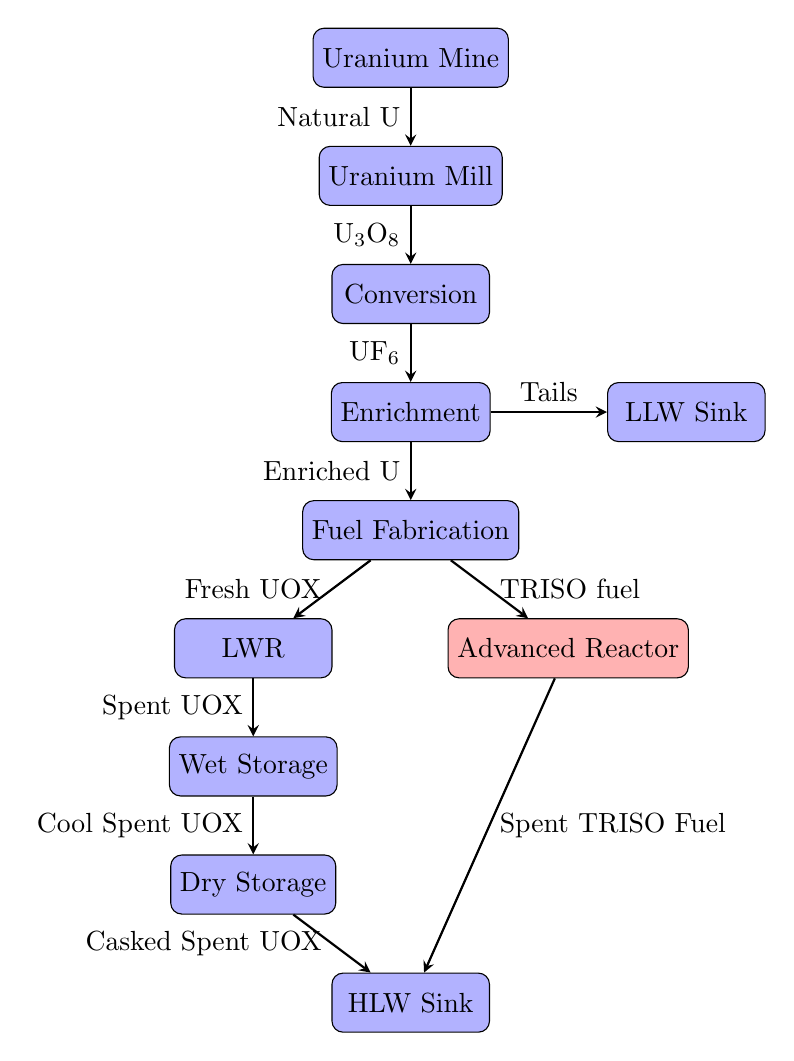
\begin{tikzpicture}[node distance=1.5cm]
            \node (mine) [facility] {Uranium Mine};
            \node (mill) [facility, below of=mine] {Uranium Mill};
            \node (conversion) [facility, below of=mill] {Conversion};
            \node (enrichment) [facility, below of=conversion]{Enrichment};
            \node (fabrication) [facility, below of=enrichment]{Fuel Fabrication};
            \node (reactor) [facility, below of=fabrication, xshift=-2cm]{LWR};
            \node (adv_reactor) [transition, below of=fabrication, xshift=2cm]{Advanced Reactor};
            \node (wetstorage) [facility, below of=reactor]{Wet Storage};
            \node (drystorage) [facility, below of=wetstorage]{Dry Storage};
            \node (sinkhlw) [facility, below of=drystorage, xshift=2cm]{HLW Sink};
            \node (sinkllw) [facility, right of=enrichment, xshift=2cm] {LLW Sink};

            \draw [arrow] (mine) -- node[anchor=east]{Natural U} (mill); 
            \draw [arrow] (mill) -- node[anchor=east]{U$_3$O$_8$}(conversion); 
            \draw [arrow] (conversion) -- node[anchor=east]{UF$_6$}(enrichment);
            \draw [arrow] (enrichment) -- node[anchor=east]{Enriched U}(fabrication);
            \draw [arrow] (enrichment) -- node[anchor=south]{Tails}(sinkllw);
            \draw [arrow] (fabrication) -- node[anchor=east]{Fresh UOX}(reactor);
            \draw [arrow] (fabrication) -- node[anchor=west]{TRISO fuel}(adv_reactor);
            \draw [arrow] (reactor) -- node[anchor=east]{Spent UOX}(wetstorage);
            \draw [arrow] (wetstorage) -- node[anchor=east]{Cool Spent UOX}(drystorage);
            \draw [arrow] (drystorage) -- node[anchor=east]{Casked Spent UOX}(sinkhlw);
            \draw [arrow] (adv_reactor) -- node[anchor=west]{Spent TRISO Fuel}(sinkhlw);

            \end{tikzpicture}
        \DIFaddendFL \caption{Fuel cycle facilities and material flow between facilities. Facilities in 
        red are deployed in the transition scenarios.}
        \label{fig:fuel_cycle}
    \end{figure}

\DIFdelbegin \DIFdel{Material compositions are defined using recipes. Spent and fresh \mbox{%DIFAUXCMD
\gls{LWR} 
}\hspace{0pt}%DIFAUXCMD
fuel recipes were obtained from \mbox{%DIFAUXCMD
\cite{yacout_visionverifiable_2006}}\hspace{0pt}%DIFAUXCMD
. The spent \mbox{%DIFAUXCMD
\gls{LWR} }\hspace{0pt}%DIFAUXCMD
fuel 
recipe assumes }\DIFdelend \DIFaddbegin \DIFadd{Recipes define the composition of the materials shown in Figure 
\ref{fig:fuel_cycle}. Yacout et al. \mbox{%DIFAUXCMD
\cite{yacout_visionverifiable_2006}
}\hspace{0pt}%DIFAUXCMD
supplied recipes for spent and fresh \mbox{%DIFAUXCMD
\gls{LWR} }\hspace{0pt}%DIFAUXCMD
fuel
assuming }\DIFaddend a 51 MWd/kg-U burnup. All other recipes capture the 
necessary \DIFdelbegin \DIFdel{isotopic ratios of uranium}\DIFdelend \DIFaddbegin \DIFadd{uranium isotopic ratios}\DIFaddend , but do not include other elements.
\DIFdelbegin \DIFdel{The enrichment feed recipe assumes natural uranium is used}\DIFdelend \DIFaddbegin \DIFadd{This work does not include neutronic or depletion simulations to determine 
any material compositions.   
The enrichment facility assumes the feed material is \mbox{%DIFAUXCMD
\gls{NU}}\hspace{0pt}%DIFAUXCMD
}\DIFaddend , 
and the tails assay is 0.2\%. 
\section{Results}
The results presented for each scenario include the energy produced, reactor 
deployment schedule, enriched
uranium mass, \gls{HALEU} mass, and \gls{SWU} capacity required as a function 
of time. 

\subsection{Scenario 1}
The \DIFdelbegin \DIFdel{amount of }\DIFdelend energy supplied by the \glspl{LWR} and the number of \glspl{LWR}
deployed as a function of time are shown in Figure \ref{fig:energy_rx_1}. 
\glspl{LWR} are first deployed in August of \DIFdelbegin \DIFdel{1967, and the }\DIFdelend \DIFaddbegin \DIFadd{1967. The }\DIFaddend last 
\gls{LWR} is deployed in June of 2016 and decommissioned in July 2076. The 
maximum number of 
\glspl{LWR} deployed at one time is 109. The energy produced by the 
\glspl{LWR} follows the number of reactors deployed. The maximum energy 
produced by the \glspl{LWR} is 102.46 GWe-y, and they produce 91.82 GWe-y 
in 2025.

\begin{figure}
    \centering 
    \DIFdelbeginFL %DIFDELCMD < \includegraphics[width=\textwidth]{figures/energy_scenario1.png}
%DIFDELCMD <     %%%
\DIFdelendFL \DIFaddbeginFL \includegraphics[width=\textwidth]{../figures/energy_scenario1.png}
    \DIFaddendFL \caption{Energy supplied by \glspl{LWR} compared to the number of 
    \glspl{LWR} deployed in Scenario 1.}
    \label{fig:energy_rx_1}
\end{figure}

Next, Figure \ref{fig:fuel_1} shows the mass of enriched uranium sent to 
the \glspl{LWR} at each time step. The \glspl{LWR} are 
defined to have an 18 month cycle length, with a third of the uranium 
mass replaced \DIFdelbegin \DIFdel{at }\DIFdelend each refueling outage. \DIFdelbegin \DIFdel{However, when a new reactor 
is deployed it is }\DIFdelend \DIFaddbegin \DIFadd{New reactors in the simulations 
are }\DIFaddend deployed with an entire core of uranium\DIFdelbegin \DIFdel{which leads 
to the large }\DIFdelend \DIFaddbegin \DIFadd{, leading 
to }\DIFaddend increases in the mass of uranium sent to the reactors \DIFaddbegin \DIFadd{at a single time 
step}\DIFaddend , such 
as in 1983 and 2016. An average of 96.2 MTU/month and a maximum of 513.7 MTU 
are sent to the \glspl{LWR}. Prior to 2025, the average mass
of enriched uranium sent to the \glspl{LWR} is 157.6 MTU/month. \DIFaddbegin \DIFadd{A total 
of 30,635.0 MTU are sent to \mbox{%DIFAUXCMD
\glspl{LWR} }\hspace{0pt}%DIFAUXCMD
after 2025 in this scenario. 
}\DIFaddend 

\begin{figure}
    \centering 
    \DIFdelbeginFL %DIFDELCMD < \includegraphics[width=\textwidth]{figures/fuelsupply_scenarios_1.png}
%DIFDELCMD <     %%%
\DIFdelendFL \DIFaddbeginFL \includegraphics[width=\textwidth]{../figures/fuelsupply_scenarios_1.png}
    \DIFaddendFL \caption{Mass of enriched uranium sent to reactors in Scenario 1.}
    \label{fig:fuel_1}
\end{figure}

Finally, \DIFaddbegin \DIFadd{Figure \ref{fig:swu_1} shows }\DIFaddend the \gls{SWU} capacity to produce 
fuel for the scenario\DIFdelbegin \DIFdel{is shown in 
Figure \ref{fig:swu_1}}\DIFdelend . The \gls{SWU} capacity required as a function of 
time follows the mass of uranium sent to the reactors, \DIFdelbegin \DIFdel{since }\DIFdelend \DIFaddbegin \DIFadd{because }\DIFaddend the \gls{SWU}
is calculated based on those transactions. \DIFdelbegin \DIFdel{An }\DIFdelend \DIFaddbegin \DIFadd{This scenario requires an 
}\DIFaddend average of 0.74$\times 10^6$ kg-\gls{SWU}/month and a maximum of 
3.95$\times 10^6$ kg-\gls{SWU}\DIFdelbegin \DIFdel{are 
required for this scenario}\DIFdelend . Prior to 2025, \DIFaddbegin \DIFadd{this scenario requires 
}\DIFaddend an average of 1.21$\times 10^6$ kg-\gls{SWU}/month \DIFaddbegin \DIFadd{to enrich the uranium 
sent to the \mbox{%DIFAUXCMD
\glspl{LWR}}\hspace{0pt}%DIFAUXCMD
.
After 2025, an average of 0.302$\times 10^6$ kg-\mbox{%DIFAUXCMD
\gls{SWU} }\hspace{0pt}%DIFAUXCMD
}\DIFaddend is required to 
enrich the uranium sent to the \glspl{LWR}.
\DIFaddbegin \DIFadd{A total of 11.1$\times 10^8$ kg-SWU are required to enrich uranium for the 
reactors in this scenario, and a total of 2.36$\times 10^8$ kg-SWU is required 
to enrich uranium sent to \mbox{%DIFAUXCMD
\glspl{LWR} }\hspace{0pt}%DIFAUXCMD
after 2025. 
}\DIFaddend 

\begin{figure}
    \centering
    \DIFdelbeginFL %DIFDELCMD < \includegraphics[width=\textwidth]{figures/totalswu_scenarios_1.png}
%DIFDELCMD <     %%%
\DIFdelendFL \DIFaddbeginFL \includegraphics[width=\textwidth]{../figures/totalswu_scenarios_1.png}
    \DIFaddendFL \caption{Total \gls{SWU} capacity required to produce fuel sent to the 
    reactors at each time step in Scenario 1.}
    \label{fig:swu_1}
\end{figure}

The \DIFaddbegin \DIFadd{other scenarios in this work apply the }\DIFaddend deployment and decommissioning 
schedule of the \glspl{LWR} in this scenario\DIFdelbegin \DIFdel{is 
applied to each of the other scenarios}\DIFdelend , and therefore the material 
requirements of \DIFdelbegin \DIFdel{each of the following scenarios }\DIFdelend \DIFaddbegin \DIFadd{the transition scenarios prior to 2025 }\DIFaddend are the 
same as those of this scenario\DIFdelbegin \DIFdel{prior to 2025. 
}\DIFdelend \DIFaddbegin \DIFadd{.  
}\DIFaddend 

\subsection{Scenario 2}
The energy produced by each type of reactor, the transition energy demand, 
and the deployment schedule of the \glspl{MMR} \DIFdelbegin \DIFdel{for }\DIFdelend \DIFaddbegin \DIFadd{in }\DIFaddend Scenario 2 are shown in 
Figure \ref{fig:energy_rx_2}. The first \glspl{MMR} are deployed in 
October 2031, and the maximum number deployed at one time is 
9,182. \DIFaddbegin \DIFadd{This is about an order of magnitude greater than the \mbox{%DIFAUXCMD
\glspl{LWR}
}\hspace{0pt}%DIFAUXCMD
deployed in 2025.
}\DIFaddend 

Once the transition begins in 2025, \DIFdelbegin \DIFdel{there are some time periods in which 
}\DIFdelend the energy demand of the scenario is 
not met \DIFaddbegin \DIFadd{every year}\DIFaddend . The first of \DIFdelbegin \DIFdel{these }\DIFdelend \DIFaddbegin \DIFadd{energy deficit }\DIFaddend is between 2030-2050, with a 
maximum deficit 
of 5.7855 GWe-y in 2032. Other periods in which the energy demand is not met 
correspond to the decommissioning of \glspl{MMR} at the end of their lifetime 
and the deployment of new reactors, such as from 2062-2069. 
The deployment of \glspl{MMR} in 2031 contributes to the inability to 
meet the energy demand of the scenario between 2030-2050, because the energy 
produced by 
\glspl{LWR} decreases to 89.35 GWe-y in 2030, despite a demand of 91.82
GWe-y, before the \DIFdelbegin \DIFdel{\mbox{%DIFAUXCMD
\glspl{MMR} }\hspace{0pt}%DIFAUXCMD
are 
deployed}\DIFdelend \DIFaddbegin \Cycamore \DIFadd{ManagerInst deploys \mbox{%DIFAUXCMD
\glspl{MMR}}\hspace{0pt}%DIFAUXCMD
}\DIFaddend .
Therefore, the \DIFdelbegin \DIFdel{reactors are deployed }\DIFdelend \DIFaddbegin \DIFadd{institution deploys the reactors }\DIFaddend in a reactionary fashion to 
past energy production, as opposed to in response to forecasted energy 
production. \DIFaddbegin \DIFadd{This deployment scheme will likely lead to an underestimation 
of fuel requirements, because the reactors are deployed at a later time 
than required by the energy demand.
}\DIFaddend 

\begin{figure}
    \centering 
    \DIFdelbeginFL %DIFDELCMD < \includegraphics[width=\textwidth]{figures/energy_scenario2.png}
%DIFDELCMD <     %%%
\DIFdelendFL \DIFaddbeginFL \includegraphics[width=\textwidth]{../figures/energy_scenario2.png}
    \DIFaddendFL \caption{Energy supplied by each type of reactor compared to the number of 
    \glspl{MMR} deployed in Scenario 2.}
    \label{fig:energy_rx_2}
\end{figure}

Next, Figure \ref{fig:fuel_2} shows the mass of enriched uranium sent to all 
reactors in the scenario and just to the \glspl{MMR}. The \glspl{MMR} 
do not require refueling during their lifetime, so uranium is  
\DIFdelbegin \DIFdel{only 
}\DIFdelend sent to these reactors \DIFaddbegin \DIFadd{only }\DIFaddend when they are deployed. \DIFdelbegin \DIFdel{This causes the 
large increases in uranium sent to these reactors and the periods of 
no uranium sent to them. An }\DIFdelend \DIFaddbegin \DIFadd{Thus, there are periods
of uranuim demand corresponding the \mbox{%DIFAUXCMD
\gls{MMR} }\hspace{0pt}%DIFAUXCMD
deployment, separated by periods
of low or no demand. All of the reactors receive an }\DIFaddend average of 104.94 
MTU/month and a maximum of 781.41 MTU \DIFdelbegin \DIFdel{are sent to all of the reactors in the scenario }\DIFdelend after 2025. 
This average is \DIFdelbegin \DIFdel{lower }\DIFdelend \DIFaddbegin \DIFadd{less }\DIFaddend than the average mass of enriched uranium 
sent to the \glspl{LWR} in Scenario 1, but the maximum \DIFaddbegin \DIFadd{sent to the \mbox{%DIFAUXCMD
\glspl{MMR}
}\hspace{0pt}%DIFAUXCMD
}\DIFaddend exceeds the maximum 
mass of enriched uranium sent to \glspl{LWR} in Scenario 1 by 267.71 \DIFdelbegin \DIFdel{MT.
An average of 48.50 }\DIFdelend \DIFaddbegin \DIFadd{MTU.
The \mbox{%DIFAUXCMD
\glspl{MMR} }\hspace{0pt}%DIFAUXCMD
receive an average of 73.12 }\DIFaddend MTU/month and a maximum of 719.25 
MTU \DIFdelbegin \DIFdel{are sent to the \mbox{%DIFAUXCMD
\glspl{MMR} }\hspace{0pt}%DIFAUXCMD
}\DIFdelend once they are deployed in 2031. The \DIFaddbegin \DIFadd{metrics for the \mbox{%DIFAUXCMD
\glspl{LWR} }\hspace{0pt}%DIFAUXCMD
after 2025
are the same as those in Scenario 1, because the \mbox{%DIFAUXCMD
\gls{LWR} }\hspace{0pt}%DIFAUXCMD
deployment and decommissioning 
scheme is the same in both scenarios.  The }\DIFaddend average 
mass of enriched uranium sent to the 
\glspl{MMR} is \DIFdelbegin \DIFdel{lower }\DIFdelend \DIFaddbegin \DIFadd{less }\DIFaddend than the average mass of uranium sent to the \glspl{LWR}
prior to 2025. This is despite a \DIFdelbegin \DIFdel{much higher }\DIFdelend \DIFaddbegin \DIFadd{greater }\DIFaddend maximum and multiple peaks \DIFdelbegin \DIFdel{higher
than }\DIFdelend \DIFaddbegin \DIFadd{larger
than the
}\DIFaddend average mass sent to the \glspl{LWR}. The \DIFdelbegin \DIFdel{lower average is explained by }\DIFdelend \DIFaddbegin \DIFadd{smaller average is because of the 
lack of refueling and }\DIFaddend the multiple time \DIFdelbegin \DIFdel{periods in 
which no \mbox{%DIFAUXCMD
\gls{HALEU} }\hspace{0pt}%DIFAUXCMD
is sent to the \mbox{%DIFAUXCMD
\glspl{MMR} }\hspace{0pt}%DIFAUXCMD
due to the lack of refueling}\DIFdelend \DIFaddbegin \DIFadd{steps when additional 
\mbox{%DIFAUXCMD
\glspl{MMR} }\hspace{0pt}%DIFAUXCMD
are not deployed. The average mass of uranium required to fuel 
the \mbox{%DIFAUXCMD
\glspl{MMR} }\hspace{0pt}%DIFAUXCMD
is more than what is required by \mbox{%DIFAUXCMD
\gls{EG} }\hspace{0pt}%DIFAUXCMD
02 
\mbox{%DIFAUXCMD
\cite{wigeland_nuclear_2014}}\hspace{0pt}%DIFAUXCMD
, despite producing less power. 
After 2025, all of the reactors receive a total of 81,747.7 MTU. The  
\mbox{%DIFAUXCMD
\glspl{MMR} }\hspace{0pt}%DIFAUXCMD
receive a total of 51,112.7 MTU. These totals show that most 
of the uranium produced after 2025 is for use in the advanced reactors, 
which is consistent with the reactor deployment and decommissioning schedule}\DIFaddend . 

\begin{figure}
    \centering
    \DIFdelbeginFL %DIFDELCMD < \begin{subfigure}{0.5\textwidth}
%DIFDELCMD <         %%%
\DIFdelendFL \DIFaddbeginFL \begin{subfigure}{0.45\textwidth}
        \DIFaddendFL \centering
        \DIFdelbeginFL %DIFDELCMD < \includegraphics[scale=0.5]{figures/fuelsupply_scenarios_2.png}
%DIFDELCMD <         %%%
\DIFdelendFL \DIFaddbeginFL \includegraphics[scale=0.4]{../figures/fuelsupply_scenarios_2.png}
        \DIFaddendFL \caption{Mass of enriched uranium sent to all reactors.}
        \label{fig:totalfuel_2}
    \end{subfigure}
    \hspace{0.8cm}
    \DIFdelbeginFL %DIFDELCMD < \begin{subfigure}{0.5\textwidth}
%DIFDELCMD <         %%%
\DIFdelendFL \DIFaddbeginFL \begin{subfigure}{0.45\textwidth}
        \DIFaddendFL \centering
        \DIFdelbeginFL %DIFDELCMD < \includegraphics[scale=0.5]{figures/advancedRX_fuelsupply_scenarios_2.png}
%DIFDELCMD <         %%%
\DIFdelendFL \DIFaddbeginFL \includegraphics[scale=0.4]{../figures/advancedRX_fuelsupply_scenarios_2.png}
        \DIFaddendFL \caption{Mass of enriched uranium sent to \glspl{MMR}.}
        \label{fig:haleu_2}
    \end{subfigure}
    \caption{\DIFdelbeginFL \DIFdelFL{Uranium }\DIFdelendFL \DIFaddbeginFL \DIFaddFL{Enriched uranium }\DIFaddendFL mass sent to reactors in Scenario 2.}
    \label{fig:fuel_2}
\end{figure}

Figure \ref{fig:swu_2} shows the \gls{SWU} capacity needed to 
enrich uranium for all reactors in the scenario, and to enrich uranium for 
just the \glspl{MMR}. \DIFdelbegin \DIFdel{There is a large difference in the \mbox{%DIFAUXCMD
\gls{SWU} 
}\hspace{0pt}%DIFAUXCMD
capacity needed to enrich uranium for \mbox{%DIFAUXCMD
\glspl{LWR} }\hspace{0pt}%DIFAUXCMD
and \mbox{%DIFAUXCMD
\glspl{MMR}}\hspace{0pt}%DIFAUXCMD
. This 
is }\DIFdelend \DIFaddbegin \DIFadd{The \mbox{%DIFAUXCMD
\gls{MMR} }\hspace{0pt}%DIFAUXCMD
fleet requires a greater \mbox{%DIFAUXCMD
\gls{SWU} 
}\hspace{0pt}%DIFAUXCMD
capacity than the \mbox{%DIFAUXCMD
\gls{LWR} }\hspace{0pt}%DIFAUXCMD
fleet 
prior to 2025 }\DIFaddend because the \glspl{MMR} require \DIFdelbegin \DIFdel{a much larger mass and 
}\DIFdelend \DIFaddbegin \DIFadd{uranium at }\DIFaddend a higher enrichment 
level. \DIFdelbegin \DIFdel{An average of 
1.37}\DIFdelend \DIFaddbegin \DIFadd{Enriching uranium for the \mbox{%DIFAUXCMD
\glspl{MMR} }\hspace{0pt}%DIFAUXCMD
requires an average of 
2.07}\DIFaddend $\times 10^6$ kg-\gls{SWU}/month and a maximum of 20.3$\times 10^6$ 
kg-\gls{SWU}\DIFdelbegin \DIFdel{are needed to enrich the uranium sent to \mbox{%DIFAUXCMD
\glspl{MMR}}\hspace{0pt}%DIFAUXCMD
}\DIFdelend . These values are both \DIFdelbegin \DIFdel{higher }\DIFdelend \DIFaddbegin \DIFadd{more }\DIFaddend than the 
average and maximum \gls{SWU} capacity needed to enrich \DIFdelbegin \DIFdel{fuel }\DIFdelend \DIFaddbegin \DIFadd{uranium }\DIFaddend for the 
\glspl{LWR} \DIFdelbegin \DIFdel{in Scenario 1. 
}\DIFdelend \DIFaddbegin \DIFadd{prior to 2025. Enriching uranium for all reactors after 2025 
requires a total of 16.8$\times 10^8$ kg-SWU. Enriching uranium for 
just the \mbox{%DIFAUXCMD
\glspl{MMR} }\hspace{0pt}%DIFAUXCMD
requires 14.4$\times 10^8$ kg-SWU. 
}\DIFaddend 

\begin{figure}
    \centering
    \DIFdelbeginFL %DIFDELCMD < \begin{subfigure}{0.5\textwidth}
%DIFDELCMD <         %%%
\DIFdelendFL \DIFaddbeginFL \begin{subfigure}{0.45\textwidth}
        \DIFaddendFL \centering
        \DIFdelbeginFL %DIFDELCMD < \includegraphics[scale=0.5]{figures/totalswu_scenarios_2.png}
%DIFDELCMD <         %%%
\DIFdelendFL \DIFaddbeginFL \includegraphics[scale=0.4]{../figures/totalswu_scenarios_2.png}
        \DIFaddendFL \caption{\DIFdelbeginFL \DIFdelFL{Total }\DIFdelendFL \gls{SWU} required to enrich uranium sent to all reactors at each time step.}
        \label{fig:totalswu_2}
    \end{subfigure}
    \hspace{0.8cm}
    \DIFdelbeginFL %DIFDELCMD < \begin{subfigure}{0.5\textwidth}
%DIFDELCMD <         %%%
\DIFdelendFL \DIFaddbeginFL \begin{subfigure}{0.45\textwidth}
        \DIFaddendFL \centering
        \DIFdelbeginFL %DIFDELCMD < \includegraphics[scale=0.5]{figures/haleuSWU_scenarios_2.png}
%DIFDELCMD <         %%%
\DIFdelendFL \DIFaddbeginFL \includegraphics[scale=0.4]{../figures/haleuSWU_scenarios_2.png}
        \DIFaddendFL \caption{\gls{SWU} required to enrich uranium sent to \glspl{MMR} at each time step.}
        \label{fig:haleuswu_2}
    \end{subfigure}
    \caption{\gls{SWU} required to enrich natural uranium in Scenario 2.}
    \label{fig:swu_2}
\end{figure}

\subsection{Scenario 3}
For Scenario 3, Figure \ref{fig:energy_rx_3} shows the number of Xe-100 
reactors deployed, the energy produced by each reactor type, and the 
energy demand. Xe-100 reactors are deployed in October 2031, which is the 
same as when \glspl{MMR}
are deployed in Scenario 2. Scenario 3 deploys a maximum of 1,225 Xe-100 
reactors\DIFdelbegin \DIFdel{.
}\DIFdelend \DIFaddbegin \DIFadd{, nine times the number of \mbox{%DIFAUXCMD
\glspl{MMR} }\hspace{0pt}%DIFAUXCMD
in Scenerio 2.
}\DIFaddend 

\DIFdelbegin \DIFdel{The }\DIFdelend \DIFaddbegin \DIFadd{Scenario 3 exhibits the }\DIFaddend same deficit between the energy produced and 
demand between 2030-2050 that was observed in Scenario \DIFdelbegin \DIFdel{2 is present in the energy produced 
in this scenario. However, there are no significant 
differences (more than 1 GWe-y for this work) between }\DIFdelend \DIFaddbegin \DIFadd{2. However, }\DIFaddend the 
energy produced \DIFdelbegin \DIFdel{and demand of the scenario 
}\DIFdelend \DIFaddbegin \DIFadd{does not differ from the energy demand by more than 1 GWe-yr 
}\DIFaddend after 2050 because the Xe-100 reactors have a longer lifetime \DIFdelbegin \DIFdel{, and there are 
no decreases in energy due to decommissioning of reactors}\DIFdelend \DIFaddbegin \DIFadd{and the 
simulation does not include the replacement of the Xe-100s}\DIFaddend . After 2050, the 
maximum difference between the energy produced and demand is 0.057 GWe-y. 

\begin{figure}
    \centering 
    \DIFdelbeginFL %DIFDELCMD < \includegraphics[width=\textwidth]{figures/energy_scenario3.png}
%DIFDELCMD <     %%%
\DIFdelendFL \DIFaddbeginFL \includegraphics[width=\textwidth]{../figures/energy_scenario3.png}
    \DIFaddendFL \caption{Energy supplied by each type of reactor compared to the number of 
    Xe-100s deployed in Scenario 3.}
    \label{fig:energy_rx_3}
\end{figure}

Comparing the mass of uranium sent to all of the reactors and just the Xe-100 
reactors, shown in Figure \ref{fig:fuel_3}, the Xe-100 reactors 
require \DIFdelbegin \DIFdel{significantly less fuel }\DIFdelend \DIFaddbegin \DIFadd{less fuel at each time step }\DIFaddend than what is sent to the \glspl{LWR}, 
despite there being more Xe-100 reactors than \glspl{LWR}. \DIFdelbegin \DIFdel{Uranium 
is sent to the Xe-100 reactors every six months in the simulations, 
while it is sent to the \mbox{%DIFAUXCMD
\glspl{LWR} }\hspace{0pt}%DIFAUXCMD
every 18 months. }\DIFdelend An average of 
74.98 MTU/month and a maximum of 342.58 MTU are sent to all of the reactors 
in this scenario starting in 2025. \DIFdelbegin \DIFdel{Both values are much
lower than in Scenario 1. }\DIFdelend An average of \DIFdelbegin \DIFdel{23.81 
}\DIFdelend \DIFaddbegin \DIFadd{39.74 
}\DIFaddend MTU/month and a maximum of 105.67 MTU are sent to the Xe-100 reactors in 
this scenario. \DIFdelbegin \DIFdel{Each of these numbers are lower }\DIFdelend \DIFaddbegin \DIFadd{Both metrics are less }\DIFaddend than the 
average and maximum masses of enriched uranium  
in Scenario 1, and the \gls{HALEU} mass sent to the \glspl{MMR} in 
Scenario 2. \DIFaddbegin \DIFadd{The average mass required to fuel the Xe-100 reactors is less 
than the fuel mass required by the \mbox{%DIFAUXCMD
\glspl{HTGR} }\hspace{0pt}%DIFAUXCMD
in \mbox{%DIFAUXCMD
\gls{EG} }\hspace{0pt}%DIFAUXCMD
02 
\mbox{%DIFAUXCMD
\cite{wigeland_nuclear_2014}}\hspace{0pt}%DIFAUXCMD
. A total of 58,410.1 MTU and 27,775.1 MTU are sent to 
all reactors after 2025 and the advanced reactors in the scenario, respectively, 
showing
that this transition scenario requires less uranium than Scenario 2. 
}\DIFaddend 

\begin{figure}
    \centering
    \DIFdelbeginFL %DIFDELCMD < \begin{subfigure}{0.5\textwidth}
%DIFDELCMD <         %%%
\DIFdelendFL \DIFaddbeginFL \begin{subfigure}{0.45\textwidth}
        \DIFaddendFL \centering
        \DIFdelbeginFL %DIFDELCMD < \includegraphics[scale=0.5]{figures/fuelsupply_scenarios_3.png}
%DIFDELCMD <         %%%
\DIFdelendFL \DIFaddbeginFL \includegraphics[scale=0.4]{../figures/fuelsupply_scenarios_3.png}
        \DIFaddendFL \caption{Mass of enriched uranium sent to all reactors.}
        \label{fig:totalfuel_3}
    \end{subfigure}
    \hspace{0.8cm}
    \DIFdelbeginFL %DIFDELCMD < \begin{subfigure}{0.5\textwidth}
%DIFDELCMD <         %%%
\DIFdelendFL \DIFaddbeginFL \begin{subfigure}{0.45\textwidth}
        \DIFaddendFL \centering
        \DIFdelbeginFL %DIFDELCMD < \includegraphics[scale=0.5]{figures/advancedRX_fuelsupply_scenarios_3.png}
%DIFDELCMD <         %%%
\DIFdelendFL \DIFaddbeginFL \includegraphics[scale=0.4]{../figures/advancedRX_fuelsupply_scenarios_3.png}
        \DIFaddendFL \caption{Mass of enriched uranium sent to Xe-100s.}
        \label{fig:haleu_3}
    \end{subfigure}
    \caption{\DIFdelbeginFL \DIFdelFL{Uranium }\DIFdelendFL \DIFaddbeginFL \DIFaddFL{Enriched uranium }\DIFaddendFL mass sent to reactors in Scenario 3.}
    \label{fig:fuel_3}
\end{figure}

Figure \ref{fig:swu_3} shows the \gls{SWU} capacity needed to enrich 
uranium for all of the reactors in the scenario, and for the uranium sent 
to just the Xe-100 reactors. \DIFdelbegin \DIFdel{There is no substantial change in the 
}\DIFdelend \DIFaddbegin \DIFadd{The average }\DIFaddend \gls{SWU} capacity needed to enrich uranium 
\DIFdelbegin \DIFdel{between Scenarios 1 and }\DIFdelend \DIFaddbegin \DIFadd{in Scenario }\DIFaddend 3 \DIFaddbegin \DIFadd{after 2025 is similar to the capacity to enrich uranium prior to 2025}\DIFaddend , 
despite the \DIFdelbegin \DIFdel{higher }\DIFdelend \DIFaddbegin \DIFadd{increased }\DIFaddend enrichment level of uranium 
sent to the Xe-100 reactors. This is because the Xe-100 reactors receive 
a \DIFdelbegin \DIFdel{lower }\DIFdelend \DIFaddbegin \DIFadd{smaller }\DIFaddend average mass of enriched uranium at each time step. Enriching uranium 
for the Xe-100 reactors requires an average of 
\DIFdelbegin \DIFdel{0.82}\DIFdelend \DIFaddbegin \DIFadd{1.37}\DIFaddend $\times 10^6$ kg-\gls{SWU}/month and a maximum of 3.64$\times 10^6$
kg-\gls{SWU}. \DIFaddbegin \DIFadd{A total of 11.9$\times 10^8$ kg-SWU and 9.57$\times 10^8$
kg-SWU are required 
to enrich uranium for all reactors after 2025 and the advanced reactors in the 
scenario, respectively. 
}\DIFaddend 

\begin{figure}
    \centering
    \DIFdelbeginFL %DIFDELCMD < \begin{subfigure}{0.5\textwidth}
%DIFDELCMD <         %%%
\DIFdelendFL \DIFaddbeginFL \begin{subfigure}{0.45\textwidth}
        \DIFaddendFL \centering
        \DIFdelbeginFL %DIFDELCMD < \includegraphics[scale=0.5]{figures/totalswu_scenarios_3.png}
%DIFDELCMD <         %%%
\DIFdelendFL \DIFaddbeginFL \includegraphics[scale=0.4]{../figures/totalswu_scenarios_3.png}
        \DIFaddendFL \caption{\gls{SWU} required to enrich uranium sent to all reactors.}
        \label{fig:totalswu_3}
    \end{subfigure}
    \hspace{0.8cm}
    \DIFdelbeginFL %DIFDELCMD < \begin{subfigure}{0.5\textwidth}
%DIFDELCMD <         %%%
\DIFdelendFL \DIFaddbeginFL \begin{subfigure}{0.45\textwidth}
        \DIFaddendFL \centering
        \DIFdelbeginFL %DIFDELCMD < \includegraphics[scale=0.5]{figures/haleuSWU_scenarios_3.png}
%DIFDELCMD <         %%%
\DIFdelendFL \DIFaddbeginFL \includegraphics[scale=0.4]{../figures/haleuSWU_scenarios_3.png}
        \DIFaddendFL \caption{\gls{SWU} required to enrich uranium sent to Xe-100s.}
        \label{fig:haleuswu_3}
    \end{subfigure}
    \caption{\gls{SWU} required to enrich natural uranium in Scenario 3.}
    \label{fig:swu_3}
\end{figure}

\subsection{Scenario 4}
Figure \ref{fig:energy_rx_4} shows the number of \glspl{MMR} deployed, the
energy produced by each type of reactor, and the energy demand of this
scenario with 1\% growth. \glspl{MMR} are deployed in January 2030, and the maximum 
number of \glspl{MMR} is 17,496. 

There is a deficit between the energy produced and  
demand from 2026-2046, with a maximum difference of 4.51 GWe-y in 2032.
There are no other times in which the energy demand is not met by a 
significant amount (more than 1 GWe-y), including when the \glspl{MMR} are 
decommissioned. After 2047 electricity is generally produced in surplus, 
up to 1.64 GWe-y. 

\begin{figure}
    \centering 
    \DIFdelbeginFL %DIFDELCMD < \includegraphics[width=\textwidth]{figures/energy_scenario4.png}
%DIFDELCMD <     %%%
\DIFdelendFL \DIFaddbeginFL \includegraphics[width=\textwidth]{../figures/energy_scenario4.png}
    \DIFaddendFL \caption{Energy supplied by each type of reactor compared to the number of 
    \glspl{MMR} deployed in Scenario 4.}
    \label{fig:energy_rx_4}
\end{figure}

Figure \ref{fig:fuel_4} shows the mass of enriched uranium sent to all the 
reactors in the scenario, and to just the \glspl{MMR} 
in the scenario. An average of 144.36 MTU/month and a maximum of 796.71 MTU
are sent to all the reactors starting in 2025 in this scenario. An average of 
\DIFdelbegin \DIFdel{75.62 }\DIFdelend \DIFaddbegin \DIFadd{113.64 }\DIFaddend MTU/month and a maximum of \DIFdelbegin \DIFdel{755.60 }\DIFdelend \DIFaddbegin \DIFadd{782.38 }\DIFaddend MTU are sent to just the \glspl{MMR}
in the scenario once they are deployed. The mass of \gls{HALEU}
required by the \glspl{MMR} in this scenario is \DIFdelbegin \DIFdel{higher }\DIFdelend \DIFaddbegin \DIFadd{more }\DIFaddend than  
in Scenario 2 due to the \DIFdelbegin \DIFdel{higher }\DIFdelend \DIFaddbegin \DIFadd{increased }\DIFaddend energy 
demand and the additional \glspl{MMR} deployed. The 
average mass of \gls{HALEU} sent to the \glspl{MMR} in this scenario is 
slightly \DIFdelbegin \DIFdel{lower }\DIFdelend \DIFaddbegin \DIFadd{less }\DIFaddend than the average mass sent to the \glspl{LWR}\DIFdelbegin \DIFdel{in Scenario 1 
due to the 
multiple time steps in which no uranium is sent to the \mbox{%DIFAUXCMD
\glspl{MMR}}\hspace{0pt}%DIFAUXCMD
}\DIFdelend \DIFaddbegin \DIFadd{. 
A total of 112,453.6 MTU and 81,818.6 MTU are required for all of the 
reactors after 2025 and the advanced reactors in the scenario, respectively}\DIFaddend . 

\begin{figure}
    \centering
    \DIFdelbeginFL %DIFDELCMD < \begin{subfigure}{0.5\textwidth}
%DIFDELCMD <         %%%
\DIFdelendFL \DIFaddbeginFL \begin{subfigure}{0.45\textwidth}
        \DIFaddendFL \centering
        \DIFdelbeginFL %DIFDELCMD < \includegraphics[scale=0.5]{figures/fuelsupply_scenarios_4.png}
%DIFDELCMD <         %%%
\DIFdelendFL \DIFaddbeginFL \includegraphics[scale=0.4]{../figures/fuelsupply_scenarios_4.png}
        \DIFaddendFL \caption{Mass of enriched uranium sent to all reactors.}
        \label{fig:totalfuel_4}
    \end{subfigure}
    \hspace{0.8cm}
    \DIFdelbeginFL %DIFDELCMD < \begin{subfigure}{0.5\textwidth}
%DIFDELCMD <         %%%
\DIFdelendFL \DIFaddbeginFL \begin{subfigure}{0.45\textwidth}
        \DIFaddendFL \centering
        \DIFdelbeginFL %DIFDELCMD < \includegraphics[scale=0.5]{figures/advancedRX_fuelsupply_scenarios_4.png}
%DIFDELCMD <         %%%
\DIFdelendFL \DIFaddbeginFL \includegraphics[scale=0.4]{../figures/advancedRX_fuelsupply_scenarios_4.png}
        \DIFaddendFL \caption{Mass of enriched uranium sent to \glspl{MMR}.}
        \label{fig:haleu_4}
    \end{subfigure}
    \caption{\DIFdelbeginFL \DIFdelFL{Uranium }\DIFdelendFL \DIFaddbeginFL \DIFaddFL{Enriched uranium }\DIFaddendFL mass sent to reactors in Scenario 4.}
    \label{fig:fuel_4}
\end{figure}

Figure \ref{fig:swu_4} shows the \gls{SWU} capacity required to 
enrich uranium for all the reactors in the scenario, and 
only for the \glspl{MMR}. For the same reasons described for 
Scenario 2, the \gls{SWU} capacity required to enrich uranium 
for the \glspl{MMR} is \DIFdelbegin \DIFdel{much higher }\DIFdelend \DIFaddbegin \DIFadd{greater }\DIFaddend than the capacity needed to 
enrich uranium for the \glspl{LWR}. An average of \DIFdelbegin \DIFdel{2.19}\DIFdelend \DIFaddbegin \DIFadd{3.21}\DIFaddend $\times 10^6$ 
kg-\gls{SWU}/month and a maximum of \DIFdelbegin \DIFdel{21.5}\DIFdelend \DIFaddbegin \DIFadd{22.1}\DIFaddend $\times 10^6$ kg-\gls{SWU}
are required to enrich the uranium that is sent to \glspl{MMR}. These values 
are \DIFdelbegin \DIFdel{higher }\DIFdelend \DIFaddbegin \DIFadd{larger }\DIFaddend than the \gls{SWU} 
capacity required to enrich uranium for the \glspl{MMR} in 
Scenario 2. The average \DIFdelbegin \DIFdel{is slightly higher }\DIFdelend \DIFaddbegin \DIFadd{\mbox{%DIFAUXCMD
\gls{SWU} }\hspace{0pt}%DIFAUXCMD
capacity to enrich uranium for 
the \mbox{%DIFAUXCMD
\glspl{MMR} }\hspace{0pt}%DIFAUXCMD
is slightly greater }\DIFaddend than the average \gls{SWU} 
capacity required to enrich uranium for the \glspl{LWR} before \DIFaddbegin \DIFadd{2025. 
A total of 25.5$\times 10^8$ kg-SWU and 23.1$\times 10^8$
kg-SWU are required to enrich uranium for all reactors after }\DIFaddend 2025 \DIFdelbegin \DIFdel{in 
Scenario 1. 
}\DIFdelend \DIFaddbegin \DIFadd{and the advanced 
reactors in the scenario, respectively. 
}\DIFaddend 

\begin{figure}
    \centering
    \DIFdelbeginFL %DIFDELCMD < \begin{subfigure}{0.5\textwidth}
%DIFDELCMD <         %%%
\DIFdelendFL \DIFaddbeginFL \begin{subfigure}{0.45\textwidth}
        \DIFaddendFL \centering
        \DIFdelbeginFL %DIFDELCMD < \includegraphics[scale=0.5]{figures/totalswu_scenarios_4.png}
%DIFDELCMD <         %%%
\DIFdelendFL \DIFaddbeginFL \includegraphics[scale=0.4]{../figures/totalswu_scenarios_4.png}
        \DIFaddendFL \caption{\gls{SWU} required to enrich uranium sent to all reactors.}
        \label{fig:totalswu_4}
    \end{subfigure}
    \hspace{0.8cm}
    \DIFdelbeginFL %DIFDELCMD < \begin{subfigure}{0.5\textwidth}
%DIFDELCMD <         %%%
\DIFdelendFL \DIFaddbeginFL \begin{subfigure}{0.45\textwidth}
        \DIFaddendFL \centering
        \DIFdelbeginFL %DIFDELCMD < \includegraphics[scale=0.5]{figures/haleuSWU_scenarios_4.png}
%DIFDELCMD <         %%%
\DIFdelendFL \DIFaddbeginFL \includegraphics[scale=0.4]{../figures/haleuSWU_scenarios_4.png}
        \DIFaddendFL \caption{\gls{SWU} required to enrich uranium sent to \glspl{MMR}.}
        \label{fig:haleuswu_4}
    \end{subfigure}
    \caption{\gls{SWU} required to enrich natural uranium in Scenario 4.}
    \label{fig:swu_4}
\end{figure}


\subsection{Scenario 5}
Figure \ref{fig:energy_rx_5} shows the number of Xe-100 reactors, the 
energy produced by each type of reactor, and the energy demand of the 
scenario. The Xe-100 reactors are deployed in January 2030, the 
same \DIFdelbegin \DIFdel{as when 
}\DIFdelend \DIFaddbegin \DIFadd{time 
}\DIFaddend \glspl{MMR} are deployed in Scenario 4. The maximum number of Xe-100 
reactors deployed in the scenario is 2,\DIFdelbegin \DIFdel{339. 
}\DIFdelend \DIFaddbegin \DIFadd{339, which is about 15,000 reactors 
fewer than the \mbox{%DIFAUXCMD
\glspl{MMR} }\hspace{0pt}%DIFAUXCMD
required to meet the same energy demand. 
}\DIFaddend 

\DIFdelbegin \DIFdel{There is a small deficit in the energy produced and }\DIFdelend \DIFaddbegin \DIFadd{The energy produced is less than the energy }\DIFaddend demand from 
2026-2046, the same \DIFdelbegin \DIFdel{as what }\DIFdelend \DIFaddbegin \DIFadd{deficit that }\DIFaddend is observed in Scenario 4. After this 
initial difference, there are no further significant (more than 
1 GWe-y) differences between 
the energy produced and demand. For most years after 2046 there 
is a surplus of energy, up to 1.64 GWe-y. 

\begin{figure}
    \centering 
    \DIFdelbeginFL %DIFDELCMD < \includegraphics[width=\textwidth]{figures/energy_scenario5.png}
%DIFDELCMD <     %%%
\DIFdelendFL \DIFaddbeginFL \includegraphics[width=\textwidth]{../figures/energy_scenario5.png}
    \DIFaddendFL \caption{Energy supplied by each type of reactor compared to the number of 
    Xe-100s deployed in Scenario 5.}
    \label{fig:energy_rx_5}
\end{figure}

Figure \ref{fig:fuel_5} shows the mass of enriched uranium sent \DIFdelbegin \DIFdel{the all }\DIFdelend \DIFaddbegin \DIFadd{to all of 
}\DIFaddend the reactors in the scenario and the \gls{HALEU} mass sent just to the 
Xe-100 reactors. There is \DIFdelbegin \DIFdel{a clear }\DIFdelend \DIFaddbegin \DIFadd{an }\DIFaddend increase in the mass of \gls{HALEU} sent 
to the Xe-100 reactors as time goes on, but this mass is still  
low compared to the mass of enriched uranium sent to the \glspl{LWR} in 
the scenario. An average of 95.46 MTU/month and a maximum of 347.28 MTU 
are sent to all of the reactors in this scenario after 2025. These 
values are both \DIFdelbegin \DIFdel{lower }\DIFdelend \DIFaddbegin \DIFadd{less }\DIFaddend than the uranium mass sent to the 
\glspl{LWR} \DIFdelbegin \DIFdel{in Scenario 1. }\DIFdelend \DIFaddbegin \DIFadd{prior to 2025. }\DIFaddend An average of 
\DIFdelbegin \DIFdel{38.11 }\DIFdelend \DIFaddbegin \DIFadd{60.73 }\DIFaddend MTU/month and a maximum of \DIFdelbegin \DIFdel{117.98 }\DIFdelend \DIFaddbegin \DIFadd{123.80 }\DIFaddend MTU are sent to the Xe-100 reactors. 
These metrics are all \DIFdelbegin \DIFdel{much lower }\DIFdelend \DIFaddbegin \DIFadd{less }\DIFaddend than what is observed 
for fueling the \glspl{MMR} in Scenario 4. \DIFaddbegin \DIFadd{A total of 74,361.76 MTU and 
43,726.74 MTU are required to fuel all reactors after 2025 and the advanced reactors 
in the scenario, respectively.
}\DIFaddend 


\begin{figure}
    \centering
    \DIFdelbeginFL %DIFDELCMD < \begin{subfigure}{0.5\textwidth}
%DIFDELCMD <         %%%
\DIFdelendFL \DIFaddbeginFL \begin{subfigure}{0.45\textwidth}
        \DIFaddendFL \centering
        \DIFdelbeginFL %DIFDELCMD < \includegraphics[scale=0.5]{figures/fuelsupply_scenarios_5.png}
%DIFDELCMD <         %%%
\DIFdelendFL \DIFaddbeginFL \includegraphics[scale=0.4]{../figures/fuelsupply_scenarios_5.png}
        \DIFaddendFL \caption{Mass of \DIFdelbeginFL \DIFdelFL{enriche }\DIFdelendFL \DIFaddbeginFL \DIFaddFL{enriched }\DIFaddendFL uranium sent to all reactors.}
        \label{fig:totalfuel_5}
    \end{subfigure}
    \hspace{0.8cm}
    \DIFdelbeginFL %DIFDELCMD < \begin{subfigure}{0.5\textwidth}
%DIFDELCMD <         %%%
\DIFdelendFL \DIFaddbeginFL \begin{subfigure}{0.45\textwidth}
        \DIFaddendFL \centering
        \DIFdelbeginFL %DIFDELCMD < \includegraphics[scale=0.5]{figures/advancedRX_fuelsupply_scenarios_5.png}
%DIFDELCMD <         %%%
\DIFdelendFL \DIFaddbeginFL \includegraphics[scale=0.4]{../figures/advancedRX_fuelsupply_scenarios_5.png}
        \DIFaddendFL \caption{Mass of enriched uranium sent to Xe-100s.}
        \label{fig:haleu_5}
    \end{subfigure}
    \caption{\DIFdelbeginFL \DIFdelFL{Uranium }\DIFdelendFL \DIFaddbeginFL \DIFaddFL{Enriched uranium }\DIFaddendFL mass sent to reactors in Scenario 5.}
    \label{fig:fuel_5}
\end{figure}

Finally, Figure \ref{fig:swu_5} shows the \gls{SWU} capacity required
to enrich the uranium sent to all of the reactors, and just the Xe-100
reactors. The \gls{SWU} capacity needed 
to enrich uranium for the Xe-100 reactors starts out at a similar 
amount as the \glspl{LWR}, but 
increases \DIFdelbegin \DIFdel{as }\DIFdelend \DIFaddbegin \DIFadd{with }\DIFaddend the energy demand and \DIFdelbegin \DIFdel{the number of reactors increases}\DIFdelend \DIFaddbegin \DIFadd{number of reacotrs}\DIFaddend . 
The \gls{SWU} capacity required to enrich uranium 
for the Xe-100 reactors becomes \DIFdelbegin \DIFdel{higher }\DIFdelend \DIFaddbegin \DIFadd{greater }\DIFaddend than the capacity 
required to enrich uranium for \glspl{LWR}, despite the Xe-100 
reactors requiring a \DIFdelbegin \DIFdel{lower }\DIFdelend \DIFaddbegin \DIFadd{lesser }\DIFaddend mass of uranium. This is \DIFdelbegin \DIFdel{due to the 
higher 
enrichment levelof the fuel for the }\DIFdelend \DIFaddbegin \DIFadd{because the 
}\DIFaddend Xe-100 \DIFdelbegin \DIFdel{reactors}\DIFdelend \DIFaddbegin \DIFadd{requires fuel at a greater enrichment level}\DIFaddend . An average of 
\DIFdelbegin \DIFdel{1.36}\DIFdelend \DIFaddbegin \DIFadd{2.09}\DIFaddend $\times 10^6$ kg-\gls{SWU}/month and a maximum of 
\DIFdelbegin \DIFdel{4.11}\DIFdelend \DIFaddbegin \DIFadd{4.26}\DIFaddend $\times 10^6$ kg-\gls{SWU} are required to enrich the uranium sent 
to the Xe-100 reactors. The average \gls{SWU} capacity 
required to enrich uranium for the Xe-100 reactors is \DIFdelbegin \DIFdel{a little }\DIFdelend lower 
than the average capacity needed to enrich uranium for the \glspl{MMR}
in Scenario 4, but the maximum capacity required for this scenario is much 
\DIFdelbegin \DIFdel{lower }\DIFdelend \DIFaddbegin \DIFadd{less }\DIFaddend than in Scenario 4. These values are slightly \DIFdelbegin \DIFdel{higher 
}\DIFdelend \DIFaddbegin \DIFadd{greater 
}\DIFaddend than what is observed to enrich uranium for the \glspl{LWR}
\DIFdelbegin \DIFdel{in Scenario 1
}\DIFdelend prior to 2025. \DIFaddbegin \DIFadd{A total of 17.4$\times 10^8$ kg-SWU and 15.1$\times 10^8$
kg-SWU are required to enrich uranium for all reactors after 2025 and the advanced 
reactors in the scenario.  
}\DIFaddend 

\begin{figure}
    \centering
    \DIFdelbeginFL %DIFDELCMD < \begin{subfigure}{0.5\textwidth}
%DIFDELCMD <         %%%
\DIFdelendFL \DIFaddbeginFL \begin{subfigure}{0.45\textwidth}
        \DIFaddendFL \centering
        \DIFdelbeginFL %DIFDELCMD < \includegraphics[scale=0.5]{figures/totalswu_scenarios_5.png}
%DIFDELCMD <         %%%
\DIFdelendFL \DIFaddbeginFL \includegraphics[scale=0.4]{../figures/totalswu_scenarios_5.png}
        \DIFaddendFL \caption{\DIFdelbeginFL \DIFdelFL{Total }\DIFdelendFL \gls{SWU} required to enrich uranium sent to all reactors at each time step.}
        \label{fig:totalswu_5}
    \end{subfigure}
    \hspace{0.8cm}
    \DIFdelbeginFL %DIFDELCMD < \begin{subfigure}{0.5\textwidth}
%DIFDELCMD <         %%%
\DIFdelendFL \DIFaddbeginFL \begin{subfigure}{0.45\textwidth}
        \DIFaddendFL \centering
        \DIFdelbeginFL %DIFDELCMD < \includegraphics[scale=0.5]{figures/haleuSWU_scenarios_5.png}
%DIFDELCMD <         %%%
\DIFdelendFL \DIFaddbeginFL \includegraphics[scale=0.4]{../figures/haleuSWU_scenarios_5.png}
        \DIFaddendFL \caption{\gls{SWU} required to enrich uranium sent to Xe-100s at each time step.}
        \label{fig:haleuswu_5}
    \end{subfigure}
    \caption{\gls{SWU} required to enrich natural uranium in Scenario 5.}
    \label{fig:swu_5}
\end{figure}

\DIFaddbegin \subsection{\DIFadd{Scenario comparisons}}
\DIFadd{The mass of uranium sent to all reactors for each scenario and to just the 
advanced reactors is shown in Figure \ref{fig:fuel_all}. Fueling the Xe-100 
reactors in Scenarios 3 and 5 requires less uranium than fueling the \mbox{%DIFAUXCMD
\glspl{LWR}
}\hspace{0pt}%DIFAUXCMD
prior to 2025
at each time step. Fueling the \mbox{%DIFAUXCMD
\glspl{MMR} }\hspace{0pt}%DIFAUXCMD
in Scenarios 2 and 4 requires the 
most uranium at any single time step, but the average uranium mass is less 
than what is required to fuel the \mbox{%DIFAUXCMD
\glspl{LWR} }\hspace{0pt}%DIFAUXCMD
prior to 2025. This is because 
of multiple time steps in which no or a small mass (less than 20 MTU) 
of uranium is sent to \mbox{%DIFAUXCMD
\glspl{MMR}}\hspace{0pt}%DIFAUXCMD
, which offset the timesteps that require 
a large mass of uranium (more than 200 MTU) are sent to the \mbox{%DIFAUXCMD
\glspl{MMR}}\hspace{0pt}%DIFAUXCMD
. 
}

\begin{figure}
    \centering
    \begin{subfigure}{0.45\textwidth}
        \centering
        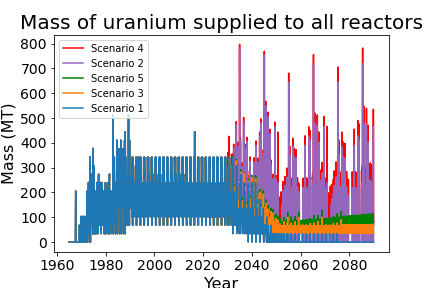
\includegraphics[scale=0.4]{../figures/fuelsupply_scenarios_all.png}
        \caption{\DIFaddFL{Total uranium mass sent to all reactors at each time step.}}
        \label{fig:totalfuel_all}
    \end{subfigure}
    \DIFaddFL{\hspace{0.8cm}
    }\begin{subfigure}{0.45\textwidth}
        \centering
        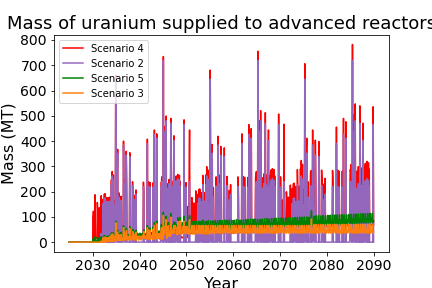
\includegraphics[scale=0.4]{../figures/advancedRX_fuelsupply_scenarios_2-5.png}
        \caption{\DIFaddFL{Uranium mass sent to advanced reactors at each time step.}}
        \label{fig:haleufuel_all}
    \end{subfigure}
    \caption{\DIFaddFL{Uranium mass supplied to reactors in all scenarios.}}
    \label{fig:fuel_all}
\end{figure}

\DIFadd{Comparing the cumulative total mass of enriched uranium required in each scenario, 
Figure \ref{fig:cumulativeU_all}, deploying the \mbox{%DIFAUXCMD
\gls{MMR} 
}\hspace{0pt}%DIFAUXCMD
requires more uranium than deploying the Xe-100 reactor for the same 
transition scenario. Figure \ref{fig:cumulativeU_all} also shows that 
deploying the \mbox{%DIFAUXCMD
\gls{MMR} }\hspace{0pt}%DIFAUXCMD
in a no growth transition 
scenario requires more uranium than deploying Xe-100 reactors in a 1\% 
growth transition for the time frame modeled. Table \ref{tab:U_summary} summarizes 
the \mbox{%DIFAUXCMD
\gls{HALEU} }\hspace{0pt}%DIFAUXCMD
mass 
requirements reported for each transition scenario: the average mass sent to 
the advanced reactors once they are deployed, the maximum mass sent to the 
advanced reactors in a single time step, and the cumulative mass sent to the 
fleet of advanced reactors for the scenario. 
}

\begin{figure}
    \centering 
    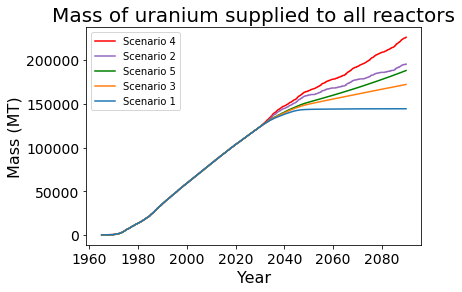
\includegraphics[scale=0.4]{../figures/fuelsupplytotal_scenarios_all.png}
    \caption{\DIFaddFL{Cumulative total uranium mass sent to all reactors in each scenario.}}
    \label{fig:cumulativeU_all}
\end{figure}


\begin{table}
    \centering
    \caption{\DIFaddFL{Summary of \mbox{%DIFAUXCMD
\gls{HALEU} }\hspace{0pt}%DIFAUXCMD
mass required in each transition scenario}}
    \label{tab:U_summary}
    \begin{tabular}{c c c c}
        \hline
        \DIFaddFL{Scenario }& \DIFaddFL{Average (MTU) }& \DIFaddFL{Max (MTU) }& \DIFaddFL{Cumulative (MTU) }\\\hline
        \DIFaddFL{2 }& \DIFaddFL{73.12 }& \DIFaddFL{719.25 }& \DIFaddFL{51,112.7 }\\
        \DIFaddFL{3 }& \DIFaddFL{39.74 }& \DIFaddFL{105.67 }& \DIFaddFL{27,775.1 }\\
        \DIFaddFL{4 }& \DIFaddFL{113.64 }& \DIFaddFL{782.38 }& \DIFaddFL{81,818.6 }\\
        \DIFaddFL{5 }& \DIFaddFL{60.73 }& \DIFaddFL{123.8 }& \DIFaddFL{43,726.4 
        }\\\hline       
    \end{tabular}
\end{table}

\DIFadd{Figure \ref{fig:swu_all} compares the \mbox{%DIFAUXCMD
\gls{SWU} }\hspace{0pt}%DIFAUXCMD
capacity required to enrich uranium for 
all reactors and the advanced reactors in each scenario. Table \ref{tab:SWU_summary} 
summarizes the \mbox{%DIFAUXCMD
\gls{SWU} }\hspace{0pt}%DIFAUXCMD
capacity 
requirements of each transition scenario: the average capacity required once the 
advanced reactors are deployed, the maximum capacity needed to enrich uranium sent to 
the advanced reactors at a single time step, and the cumulative capacity used to enrich 
uranium for the fleet of advnaced reactors. The \mbox{%DIFAUXCMD
\gls{SWU} }\hspace{0pt}%DIFAUXCMD
capacity required 
to enrich uranium in Scenarios 1, 3, and 5 are similar in magnitude. Scenarios 2 and 4
appear to require a greater \mbox{%DIFAUXCMD
\gls{SWU} }\hspace{0pt}%DIFAUXCMD
capacity because the calculated \mbox{%DIFAUXCMD
\gls{SWU} }\hspace{0pt}%DIFAUXCMD
capacity 
is based on the mass of uranium sent to the reactors at each time step. Therefore, 
the values presented do not reflect the required \mbox{%DIFAUXCMD
\gls{SWU} }\hspace{0pt}%DIFAUXCMD
capacity of 
an enrichment facility. 
}

\begin{figure}
    \centering
    \begin{subfigure}{0.45\textwidth}
        \centering
        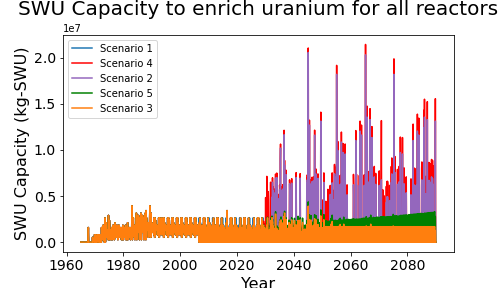
\includegraphics[scale=0.4]{../figures/totalswu_scenarios_all.png}
        \caption{\DIFaddFL{Total \mbox{%DIFAUXCMD
\gls{SWU} }\hspace{0pt}%DIFAUXCMD
required to enrich uranium sent to all reactors at each time step.}}
        \label{fig:totalswu_all}
    \end{subfigure}
    \DIFaddFL{\hspace{1.8cm}
    }\begin{subfigure}{0.45\textwidth}
        \centering
        \includegraphics[scale=0.4]{../figures/haleuSWU_scenarios_all.png}
        \caption{\DIFaddFL{\mbox{%DIFAUXCMD
\gls{SWU} }\hspace{0pt}%DIFAUXCMD
required to enrich uranium sent to advanced reactors at each time step.}}
        \label{fig:haleuswu_al}
    \end{subfigure}
    \caption{\DIFaddFL{\mbox{%DIFAUXCMD
\gls{SWU} }\hspace{0pt}%DIFAUXCMD
required to enrich natural uranium in all scenarios.}}
    \label{fig:swu_all}
\end{figure}

\begin{table}
    \centering
    \caption{\DIFaddFL{Summary of \mbox{%DIFAUXCMD
\gls{SWU} }\hspace{0pt}%DIFAUXCMD
capacity requirements in each transition scenario}}
    \label{tab:SWU_summary}
    \begin{tabular}{c c c c}
        \hline
        \DIFaddFL{Scenario }& \DIFaddFL{Average (kg-SWU) }& \DIFaddFL{Max (kg-SWU) }& \DIFaddFL{Cumulative  (kg-SWU) }\\\hline
        \DIFaddFL{2 }& \DIFaddFL{2.07$\times 10^6$ }& \DIFaddFL{20.3$\times 10^6$ }& \DIFaddFL{14.4$\times 10^8$ }\\
        \DIFaddFL{3 }& \DIFaddFL{1.37$\times 10^6$ }& \DIFaddFL{3.64$\times 10^6$ }& \DIFaddFL{9.57$\times 10^8$ }\\
        \DIFaddFL{4 }& \DIFaddFL{3.21$\times 10^6$ }& \DIFaddFL{22.1$\times 10^6$ }& \DIFaddFL{23.1$\times 10^8$ }\\
        \DIFaddFL{5 }& \DIFaddFL{2.09$\times 10^6$ }& \DIFaddFL{4.26$\times 10^6$ }& \DIFaddFL{15.1$\times 10^8$
        }\\\hline       
    \end{tabular}
\end{table}

\DIFadd{An example of a possible facility for enriching uranium for the \mbox{%DIFAUXCMD
\glspl{MMR} }\hspace{0pt}%DIFAUXCMD
in 
Scenario 2 would 
have a throughput of 66 MTU/month, and a \mbox{%DIFAUXCMD
\gls{SWU} }\hspace{0pt}%DIFAUXCMD
capacity of 2.28$\times 10^6$
kg-SWU/month. A facility of this size and capacity would be able to meet the 
enriched uranium demand, as Figure \ref{fig:enrich_storage}
shows. In this scenario, the enrichment facility goes online in 2025 and operates 
through 2090. The stored enriched uranium mass at the facility never goes below 0, 
but this example does not 
account for any time required to fabricate the fuel before shipment to the reactor.
This theoretical example shows how a constant-capacity \mbox{%DIFAUXCMD
\gls{HALEU} }\hspace{0pt}%DIFAUXCMD
enrichment 
facility can meet the enriched uranium requirements of the scenario, but further 
optimization of such a facility or the exploration of how other methods can be
used meet the enriched uranium demand is left to future work. 
}

\begin{figure}
    \centering
    \includegraphics[width=\textwidth]{../figures/potential_uranium_stockpile.png}
    \caption{\DIFaddFL{Net enriched uranium mass stored at a theoretical enrichment facility with 
    a mass throughput of 66 MTU/month. This model assumes the facility goes online in 2025
    and does not account for any time required for fuel fabrication.}}
    \label{fig:enrich_storage}
\end{figure}

\DIFaddend \section{\DIFdelbegin \DIFdel{Conclusion}\DIFdelend \DIFaddbegin \DIFadd{Conclusions}\DIFaddend }
This work simulated multiple fuel cycle scenarios to compare the 
material requirements of deploying different advanced reactors fueled 
by \gls{HALEU}. Scenarios include a no-growth and a 1\% growth 
transitions to either the \gls{USNC} \gls{MMR} or the X-energy Xe-100 
reactor from the current fleet of \DIFdelbegin \DIFdel{\mbox{%DIFAUXCMD
\glspl{LWR} }\hspace{0pt}%DIFAUXCMD
in the US. The }\DIFdelend \DIFaddbegin \DIFadd{U.S. \mbox{%DIFAUXCMD
\glspl{LWR}}\hspace{0pt}%DIFAUXCMD
. We used the }\DIFaddend current 
fleet of \glspl{LWR}, without a transition to an advanced reactor 
\DIFdelbegin \DIFdel{, is 
also simulated}\DIFdelend \DIFaddbegin \DIFadd{fleet for 
comparison}\DIFaddend . Each of these scenarios are compared for their material 
requirements, specifically the number of reactors deployed, the mass 
of enriched uranium sent to the reactors, and the \gls{SWU} capacity 
required to enrich natural uranium to produce the fuel needed for 
each scenario. 

\DIFaddbegin \DIFadd{More \mbox{%DIFAUXCMD
\glspl{MMR} }\hspace{0pt}%DIFAUXCMD
are required than Xe-100 reactors to meet the same 
energy demand, because of the differences in their power output. 
}\DIFaddend The transition scenarios exhibit some gaps between  
energy production and demand, localized to the beginning of the 
transition
scenarios, and to the replacement of \glspl{MMR} as they are decommissioned. 
Xe-100 reactors are not decommissioned in the simulated time frame because 
their lifetime exceeds the time span simulated. Therefore, the 
energy produced and the material requirements for the replacement of 
Xe-100 reactors is not explored in this work. 

\DIFdelbegin \DIFdel{This work shows that transitioning }\DIFdelend \DIFaddbegin \DIFadd{Transitioning }\DIFaddend to the \gls{MMR} requires 
a \DIFdelbegin \DIFdel{higher }\DIFdelend \DIFaddbegin \DIFadd{larger }\DIFaddend average mass and \gls{SWU} capacity than transitioning to the 
Xe-100 reactors\DIFdelbegin \DIFdel{, but a lower average than what is required by the current 
\mbox{%DIFAUXCMD
\glspl{LWR}}\hspace{0pt}%DIFAUXCMD
}\DIFdelend . Transitioning to the \gls{MMR} \DIFdelbegin \DIFdel{shows large variability in 
the mass of enriched uranium and required \mbox{%DIFAUXCMD
\gls{SWU} }\hspace{0pt}%DIFAUXCMD
capacity , because \mbox{%DIFAUXCMD
\glspl{MMR} }\hspace{0pt}%DIFAUXCMD
require a large mass of enriched uranium when they are 
first deployed and do not require refueling. This behavior is not observed 
in the transitions to }\DIFdelend \DIFaddbegin \DIFadd{requires a smaller average 
uranium mass but a greater \mbox{%DIFAUXCMD
\gls{SWU} }\hspace{0pt}%DIFAUXCMD
capacity than fueling \mbox{%DIFAUXCMD
\glspl{LWR} }\hspace{0pt}%DIFAUXCMD
prior 
to 2025 because the \mbox{%DIFAUXCMD
\gls{MMR} }\hspace{0pt}%DIFAUXCMD
requires a higher enrichment level. 
Fueling \mbox{%DIFAUXCMD
\glspl{MMR} }\hspace{0pt}%DIFAUXCMD
involves large, one-time shipments of fuel, while 
fueling }\DIFaddend the Xe-100 \DIFdelbegin \DIFdel{reactor because this reactor utilizes 
on-line refueling, so fuel 
is continually sent to them}\DIFdelend \DIFaddbegin \DIFadd{involves small, continuous shipments of fuel 
because of the different refueling schemes}\DIFaddend .

\section{Future Work}
One possible area of future work is extending the end date 
of the scenarios to 2125 to investigate how replacing deployed Xe-100 
reactors impacts the material requirements and energy produced in those 
transition scenarios. Another area of future work is to investigate the 
\DIFdelbegin \DIFdel{amount of \mbox{%DIFAUXCMD
\gls{HEU} }\hspace{0pt}%DIFAUXCMD
required to produce the \mbox{%DIFAUXCMD
\gls{HALEU} }\hspace{0pt}%DIFAUXCMD
required by each of the transitions. This will provide insight into how this \mbox{%DIFAUXCMD
\gls{HALEU} }\hspace{0pt}%DIFAUXCMD
production method can be used }\DIFdelend \DIFaddbegin \DIFadd{material requirements if the \mbox{%DIFAUXCMD
\gls{HALEU} }\hspace{0pt}%DIFAUXCMD
demand is met by downblending 
\mbox{%DIFAUXCMD
\gls{HEU} }\hspace{0pt}%DIFAUXCMD
or enriching uranium of non-natural enrichment, such as 
\mbox{%DIFAUXCMD
\gls{LEU} }\hspace{0pt}%DIFAUXCMD
below 5\% $^{235}$U. Finally, an investigation into the 
optimization of an enrichment facility or the use of other methods to 
create \mbox{%DIFAUXCMD
\gls{HALEU} }\hspace{0pt}%DIFAUXCMD
}\DIFaddend to meet the \DIFdelbegin \DIFdel{material requirements of these 
transition scenarios}\DIFdelend \DIFaddbegin \DIFadd{demand of each scenario will provide 
insight into the logistics of transitioning to \mbox{%DIFAUXCMD
\gls{HALEU}}\hspace{0pt}%DIFAUXCMD
-fueled 
reactors}\DIFaddend . 

\section{Acknowledgments}
This material is based upon work supported under an Integrated University Program Graduate
Fellowship.

The authors would like to thank Nathan Ryan of the University of Illinois 
Urbana-Champaign for his assistance in technical editing.

\bibliography{../bibliography.bib}


% Prof. Huff discourages appendices in journal articles.
% But, if you must, include one like so:
%\pagebreak
%
\appendix
\section{}


\end{document}
